%!TEX root = /Users/louis/Documents/PhD/Deliverables/Thesis/thesis.tex

\chapter{Evaluation}
\label{Evaluation}
This chapter evaluates the structures and processes proposed in this thesis with respect to the research hypothesis outlined in Section~\ref{sec:hypothesis}. In particular, the evaluation explores the extent to which the structures and processes affect developer productivity for co-evolution. As discussed in Chapter~\ref{Introduction}, 
these two characteristics are key to the success of the large and complicated software engineering projects demanded by society today. Given the time constraints of a doctoral thesis, the proposed structures and processes are prototypes, and unlikely to be fit for industrial use in their current state. The evaluation aims to determine areas in which the proposed structures and processes might be usefully improved by identifying factors that affect their efficacy. The conclusions drawn in this chapter identify benefits and drawbacks of using the proposed structures and processes for managing co-evolution in contemporary MDE development environments and for industrial software-engineering projects.

Chapter~\ref{Analysis} identified \emph{user-driven co-evolution}, a process for managing co-evolution, that had been used in real-world MDE projects and that had not been recognised in the literature. Chapter~\ref{Implementation} described the implementation of two structures tailored for user-driven co-evolution, a \emph{metamodel-independent syntax} and a \emph{textual modelling notation}. Using a real-world example of user-driven co-evolution, Section~\ref{sec:exemplar_user-driven_co-evo} assesses the extent to which the dedicated structures proposed in Chapter~\ref{Implementation} affect the productivity of user-driven co-evolution.

The remainder of the chapter evaluates developer-driven co-evolution (in which a migration strategy is specified in an executable format) and focuses on \emph{Epsilon Flock} (Section~\ref{sec:flock}), a transformation language tailored for model migration. Section~\ref{sec:quantitive} evaluates the novel source-target relationship strategy implemented in Flock, \emph{conservative copy}, by comparison with two existing source-target relationship strategies using co-evolution examples from real-world projects. Sections~\ref{sec:collaborative_comparison} and~\ref{sec:ttc} evaluate Flock as a whole, using an expert evaluation and a transformation contest, respectively. The transformation contest was judged by members of the MDE community, providing an opportunity for Flock and other transformation tools to be assessed in a peer review.

The work presented in this chapter has been published in \cite{rose10comparison,rose10ttc_solution,rose10ttc_case}. The evaluation described in Sections~\ref{sec:collaborative_comparison} and \ref{sec:ttc} was performed collaboratively, and the contributions of others are highlighted in those sections.

%!TEX root = /Users/louis/Documents/PhD/Deliverables/Thesis/thesis.tex

\section{Evaluating User-Driven Co-Evolution}
\label{sec:exemplar_user-driven_co-evo}
Several real-world MDE projects in which user-driven co-evolution has been observed were reported in Chapter~\ref{Analysis}, and Chapters~\ref{LiteratureReview} and~\ref{Analysis} highlighted that no tool support for user-driven co-evolution has yet been reported in the literature. To address this, Chapter~\ref{Implementation} proposed two structures to support user-driven co-evolution, a metamodel-independent syntax (Section~\ref{sec:mmi_syntax}) and a textual modelling notation (Section~\ref{sec:notation}). This section explores the extent to which the two structures increase the productivity of user-driven co-evolution, supporting the research hypothesis which stated that \emph{integrating dedicated structures and processes with contemporary MDE environments is beneficial in terms of increased productivity}.

To explore the hypothesis, several approaches to evaluation could be used. The metamodel-independent syntax and textual modelling notation are freely available as part of Epsilon, a component of the Eclipse Modeling Project, so the productivity benefits of the structures could have been explored by gathering and analysing the opinion of users. However, this approach was discounted because drawing meaningful conclusions would have needed understanding of each user's domain, context and background. Evaluation could have been performed with a comprehensive user study that measured the time taken for developers to perform model migration with and without the dedicated structures for user-driven co-evolution. However, locating developers and co-evolution examples was not possible in the available time. Instead, evaluation was conducted by comparing two approaches to user-driven co-evolution using an example from a real-world MDE project. The first approach uses only the tools available in the Eclipse Modeling Framework (EMF); while the second approach uses EMF together with the metamodel-independent syntax and textual modelling notation introduced in Chapter~\ref{Implementation}.

Section~\ref{subsec:challenges_for_performing_user-driven_co-evo} summarises Section~\ref{subsec:user-driven_co-evolution}, which described the challenges to productivity faced by developers while performing user-driven co-evolution with EMF. Section~\ref{subsec:user-driven_co-evolution_example} introduces the example of user-driven co-evolution used to perform the evaluation. In Sections~\ref{subsec:user-driven_co-evolution_with_emf} and~\ref{subsec:user-driven_co-evolution_with_dedicated_structures}, the two approaches to user-driven co-evolution are demonstrated. The section concludes by comparing the two approaches and highlighting ways in which the metamodel-independent syntax and textual modelling notation increase developer productivity in the context of user-driven co-evolution.

\subsection{Challenges for Performing User-Driven Co-Evolution}
\label{subsec:challenges_for_performing_user-driven_co-evo}
Two productivity challenges for performing user-driven co-evolution in contemporary MDE environments were identified in Section~\ref{subsec:user-driven_co-evolution}. Firstly, model storage representations are not optimised for use by humans, and so user-driven co-evolution -- which typically involves changing models by hand -- is made error-prone and time consuming. Secondly, the multi-pass parsers used to load models in contemporary MDE environments make user-driven co-evolution an iterative process, because not all conformance errors are reported in the first pass. The identification of these productivity challenges led to the derivation of the following research requirement in Section~\ref{sec:requirements_identification}: \emph{This thesis must demonstrate a user-driven co-evolution process that enables the editing of non-conformant models without directly manipulating the underlying storage representation and provides a conformance report for the original model and evolved metamodel.}

Two of the structures presented in Chapter~\ref{Implementation} provide the foundation for fulfilling the above research requirement. The first, a metamodel-independent syntax, facilitates the conformance checking of a model against any metamodel. The second structure, the textual modelling notation \emph{Epsilon HUTN}, allows models to be managed in a format that is reputedly easier for humans to use than XMI, the canonical model storage format \cite{hutn}.

To fulfil the above research requirement, this section uses the metamodel-independent syntax and the textual modelling notation to demonstrate that user-driven co-evolution can be performed without encountering the challenges to productivity described above. To this end, an example of co-evolution is used to show the way in which user-driven co-evolution might be achieved with and without the metamodel-independent syntax and Epsilon HUTN.

\subsection{Co-Evolution Example}
\label{subsec:user-driven_co-evolution_example}
The evaluation uses the co-evolution example taken from collaborative work with Adam Sampson, then a Research Associate at the University of Kent. The purpose of the collaboration was to build a prototypical editor for graphical models of programs written in process-oriented programming languages, such as occam-$\pi$ \cite{occam_pi}. The graphical models would provide a standard notation for describing process-oriented programs. Part of the example was used to describe Epsilon Flock in \ref{subsec:flock_examples}.

The collaboration with Sampson was selected for the evaluation presented here for several reasons. Firstly, \cc the work involved constructing a graphical model editor, which is a common MDE development activity \cite{amyot06evaluation}. Secondly, the editor was developed in an incremental and iterative manner, and involved several different types of change to the metamodel, some of which affected conformance. Finally, a relatively small number of models were constructed during the collaboration, and hence a user-driven approach to managing co-evolution was more suitable than a developer-driven approach for this example.

The graphical model editor was developed using a MDE approach. A metamodel captures the abstract syntax of process-oriented programming languages, and code for a graphical model editor is automatically generated from the metamodel. 

The final version of the graphical model editor is shown in Figure~\ref{fig:po_final_graphical_editor}. The editor captures the three primary concepts used to specify process-oriented programs: processes, connection points and channels. Processes, represented as boxes in the graphical notation, are the fundamental building blocks of a process-oriented program. Channels, represented as lines in the graphical notation, are the mechanism by which processes communicate, and are unidirectional. Connection points, represented as circles in the graphical notation, define the channels on which a process can communicate. Because channels are unidirectional, connection points are either reading (consume messages from the channel) or writing (generate messages on the channel). Reading (writing) connection points are represented as white (black) circles in the graphical notation.  

\begin{figure}[htbp]
	\centering
	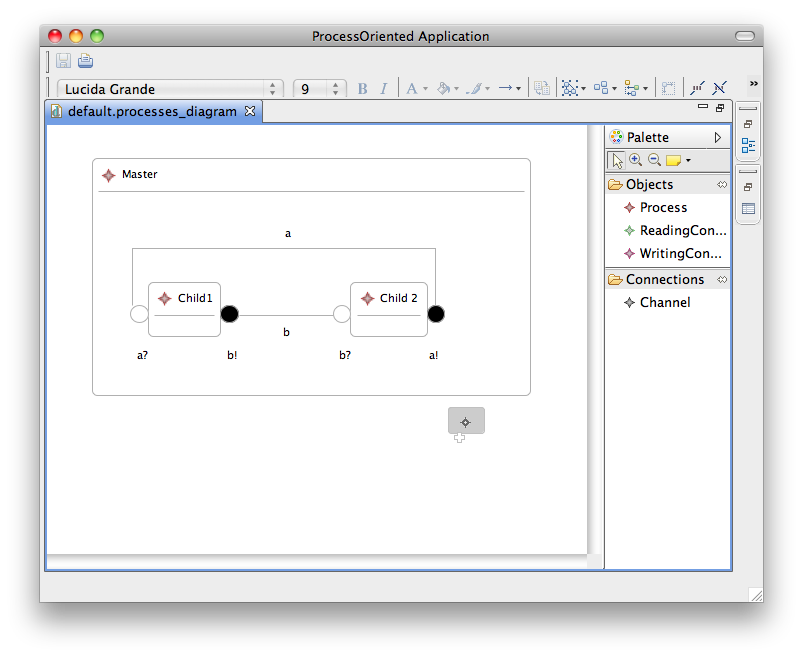
\includegraphics[width=13.5cm]{6.Evaluation/images/user_driven/po_final_editor.png}
	\caption{Final version of the prototypical graphical model editor.}
	\label{fig:po_final_graphical_editor}
\end{figure}

The graphical model editor was implemented using EMF. The metamodel was specified in Ecore, the metamodelling language of EMF, and the graphical editor was generated from the metamodel using GMF. Section~\ref{sec:mde_tools} describes in more detail the way in which EMF and GMF can be used to specify metamodels and to generate graphical model editors.

The process-oriented metamodel was developed iteratively, and the six iterations are described in Appendix~\ref{ProcessOriented}. During each iteration, the metamodel was changed. The evaluation described here uses an example of metamodel changes from the fifth iteration of the project. The way in which development proceeded during that iteration is described in Section~\ref{sec:po_it5} and summarised below.

\subsubsection{Aim of Iteration 5}
Iteration 5 of the process-oriented example was used to describe Epsilon Flock in \ref{subsec:flock_examples}. The purpose of the iteration was to refine the way in which connection points were represented. At the start of the iteration, the graphical model editor could be used to draw processes, channels and connection points. However, no distinction was made between reading and writing connection points.

Figure~\ref{fig:po_original_editor} shows a model represented in the graphical model editor before the iteration began. The model contains two processes (depicted as boxes), \texttt{P1} and \texttt{P2}, one channel (depicted as a line), \texttt{a}, and two connection points (depicted as circles), \texttt{a!} and \texttt{a?}.

\begin{figure}[htbp]
	\centering
	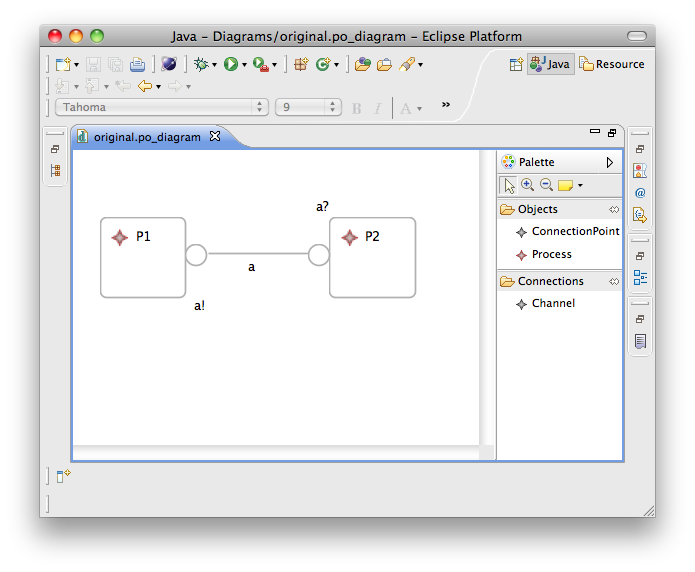
\includegraphics[width=13.5cm]{6.Evaluation/images/user_driven/po_original_editor.png}
	\caption{The graphical editor at the start of the iteration.}
	\label{fig:po_original_editor}
\end{figure}


The aim of the iteration was to distinguish between reading and writing connection points in the graphical notation. The former are used to receive messages, and the latter to send messages. In Figure~\ref{fig:po_original_editor}, \texttt{a?} is intended to represent a reading connection point, and \texttt{a!} a writing connection point. Sampson and I decided that the editor should be changed so that black circles would be used to represent writing connection points, and white circles to represent reading connection points. At the end of the iteration the model shown in Figure~\ref{fig:po_original_editor} would be represented as shown in Figure~\ref{fig:po_evolved_editor}. Furthermore, the editor would ensure that \texttt{a?} was used only as the reader of a channel, and \texttt{a!} only as the writer of a channel. Before the iteration started, the editor did not enforce this constraint.

\begin{figure}[htbp]
	\centering
	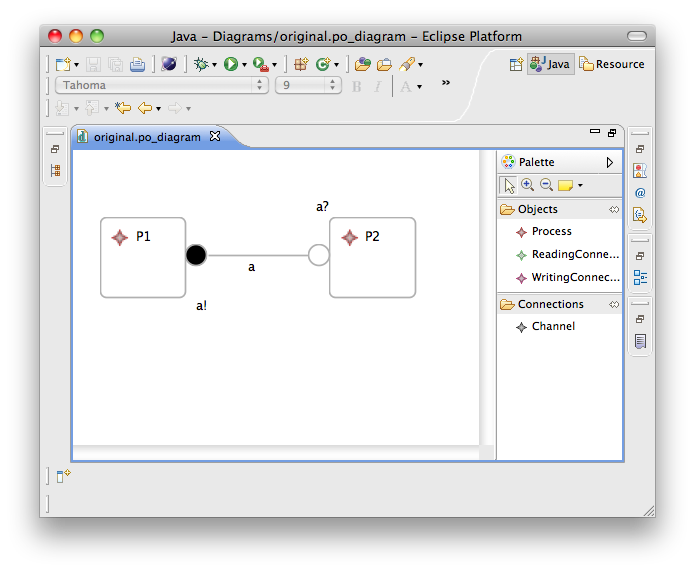
\includegraphics[width=13.5cm]{6.Evaluation/images/user_driven/po_evolved_editor.png}
	\caption{The graphical editor at the end of the iteration.}
	\label{fig:po_evolved_editor}
\end{figure}


\subsubsection{Metamodel changes during Iteration 5}
Before the iteration started, the metamodel, shown in Figure~\ref{fig:po_original_mm}, did not distinguish between reading and writing \texttt{Co\-nn\-ec\-ti\-o\-nPo\-i\-nt}s. A \texttt{Co\-nn\-ec\-ti\-o\-nPo\-i\-nt} could be associated with a \texttt{Ch\-an\-nel} via the \texttt{re\-ad\-er} or \texttt{wr\-it\-er} reference of \texttt{Ch\-an\-nel}, but the type of a \texttt{Co\-nn\-ec\-ti\-o\-nPo\-i\-nt} was not specified explicitly.

The way in which connection points were modelled was changed, resulting in the metaclasses shown in Figure~\ref{fig:po_evolved_mm}. \texttt{Co\-nn\-ec\-ti\-o\-nPo\-i\-nt} was made abstract, and two subtypes, \texttt{Re\-ad\-i\-ngCo\-nn\-ec\-ti\-o\-nPo\-i\-nt} and \texttt{Wr\-i\-ti\-ngCo\-nn\-ec\-ti\-o\-nPo\-i\-nt}, were introduced. The \texttt{re\-ad\-er} and \texttt{wr\-it\-er} references of \texttt{Ch\-an\-n\-el} were changed to refer to the new subtypes. The evolved metamodel correctly prevented the use of a \texttt{Co\-nn\-ec\-ti\-o\-nPo\-i\-nt} as both a \texttt{re\-ad\-er} and a \texttt{wr\-it\-er}.

\begin{figure}[htbp]
	\centering
	\subfigure[Part of the original metamodel.]
	{
	    \label{fig:po_original_mm}
	    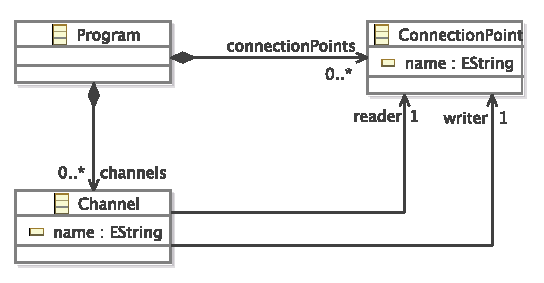
\includegraphics[width=7.5cm]{6.Evaluation/images/user_driven/po_before.pdf}
	}
	\subfigure[Part of the evolved metamodel.]
	{
	    \label{fig:po_evolved_mm}
	    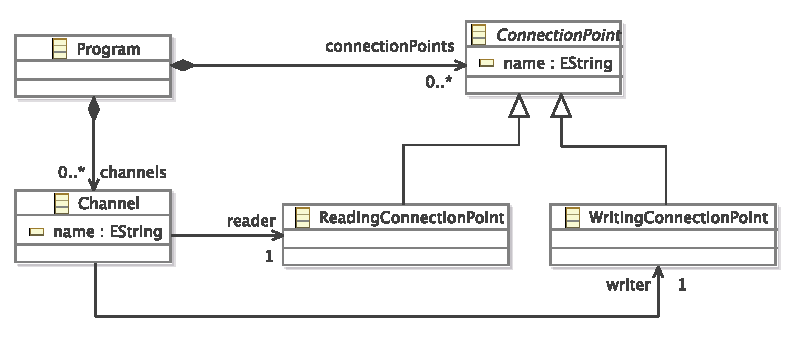
\includegraphics[width=11cm]{6.Evaluation/images/user_driven/po_after.pdf}
	}
	\caption{Process-oriented metamodel evolution.}
\label{fig:po_mms}
\end{figure}

Following the metamodel changes, a new version of the graphical editor was generated automatically from the metamodel using GMF. An annotation -- not shown in Figure~\ref{fig:po_evolved_mm} -- on the \texttt{Wr\-i\-ti\-ngCo\-nn\-ec\-ti\-o\-nPo\-i\-nt} class was used to indicate to GMF that black circles were to be used to represent writing connection points in the graphical notation.

\subsubsection{Testing during Iteration 5}
Testing the new version of the graphical editor highlighted the need for model migration. Attempting to load existing models, such as the one shown in Figure~\ref{fig:po_original_editor}, caused an error because \texttt{Co\-nn\-ec\-ti\-onP\-oi\-nt} was now an abstract class. Any model specifying at least one connection point no longer conformed to the metamodel. Model migration was performed to re-establish conformance and to allow the models to be loaded. 

Several models, presented in Appendix~\ref{ProcessOriented}, had been constructed when testing previous versions of the graphical editor. The models were used during each iteration to ensure that any changes had not introduced regressions. After the metamodel changes described above, the test models could no longer be loaded and required migration. A developer-driven co-evolution approach was not suitable for the development of process-oriented editor because only a few small models required migration in each iteration. A user-driven co-evolution approach was used instead, but, as no structures dedicated to user-driven co-evolution were available, co-evolution was performed by manually editing the storage representation of models. 

The sequel describes the way in which migration was performed during the development of the process-oriented metamodel, without dedicated structures for performing user-driven co-evolution. Section~\ref{subsec:user-driven_co-evolution_with_dedicated_structures} describes the way in which migration could have been performed using two of the structures presented in Chapter~\ref{Implementation}. The section concludes by comparing the two approaches.

\subsection{User-Driven Co-Evolution with EMF}
\label{subsec:user-driven_co-evolution_with_emf}
During the development of the process-oriented metamodel, no dedicated structures for performing user-driven co-evolution were available. Instead, migration was performed using only those tools available in EMF, as described below.

Migration with EMF involved identifying and fixing conformance errors, using the workflow shown in Figure~\ref{fig:emf_process}. The workflow was first discussed in Chapter~\ref{Analysis}. When the user attempts to load a model, EMF automatically checks the conformance of the model. If the model does not conform to its metamodel, loading fails. To re-establish conformance, the user must edit by hand the underlying storage representation of the model, XMI. Recall that co-evolution is an iterative process because EMF uses a multi-pass XMI parser and cannot report all categories of conformance problem in the first pass.

One of the test models, shown in Figure~\ref{fig:po_original_editor}, is now used to illustrate the way in which user-driven co-evolution was performed using the workflow shown in Figure~\ref{fig:emf_process}. For the test model shown in Figure~\ref{fig:po_original_editor}, the conformance problems shown in the bottom pane (and by the error markers in the left-hand margin of the top pane) of Figure~\ref{fig:po_original_xmi} were reported by EMF. For example, the first conformance problem reported is shown in the tooltip in Figure~\ref{fig:po_original_xmi}, and states that a \texttt{ClassNotFoundException} was encountered because the ``Class `ConnectionPoint' is not found or is abstract.''

\begin{figure}[htbp]
	\centering
		\includegraphics*[viewport=80 280 600 550,height=5.75cm]{6.Evaluation/images/user_driven/emf_process.pdf}
	\caption{User-driven co-evolution with EMF}
	\label{fig:emf_process}
\end{figure}

\begin{figure}[htbp]
	\centering
	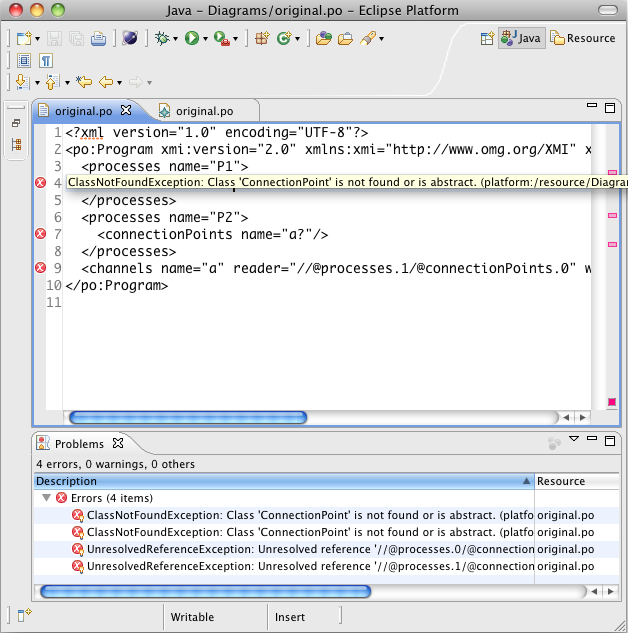
\includegraphics[width=13.5cm]{6.Evaluation/images/user_driven/po_original_xmi.png}
	\caption{XMI prior to migration}
	\label{fig:po_original_xmi}
\end{figure}

The conformance problems were fixed by editing the XMI shown in Figure~\ref{fig:po_original_xmi}, producing the XMI shown in Figure~\ref{fig:po_migrated_xmi}. The type of each connection point element was changed to either \texttt{Re\-ad\-i\-ngCo\-nn\-ec\-ti\-o\-nPo\-i\-nt} or \texttt{Wr\-i\-ti\-ngCo\-nn\-ec\-ti\-o\-nPo\-i\-nt}. The former was used when the connection point was referenced via the \texttt{reader} reference of \texttt{Channel}, and the latter otherwise. The reconciled XMI is shown in Figure~\ref{fig:po_migrated_xmi}. On lines 4 and 7, the connection point model elements have been changed to include \texttt{xsi:type} attributes, which specify whether the connection point should instantiate \texttt{Re\-ad\-i\-ngCo\-nn\-ec\-ti\-o\-nPo\-i\-nt} or \texttt{Wr\-i\-ti\-ngCo\-nn\-ec\-ti\-o\-nPo\-i\-nt}.

\begin{figure}[htbp]
	\centering
	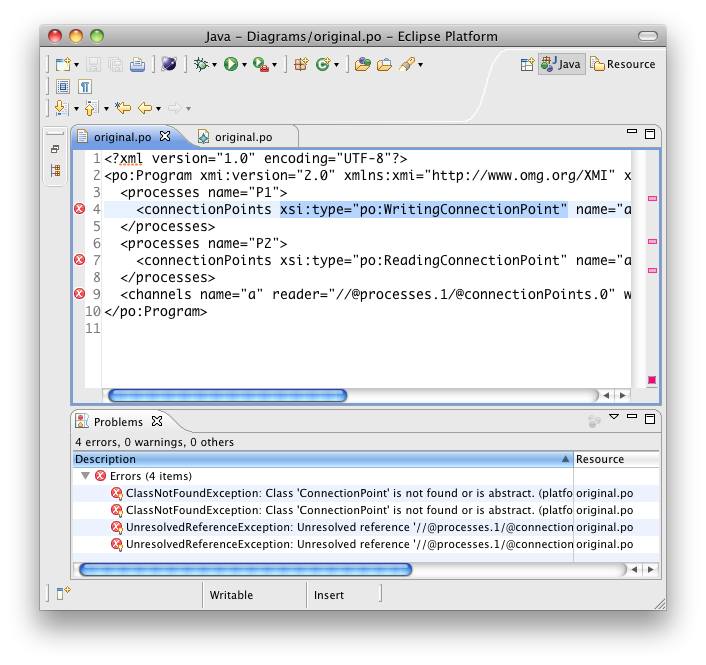
\includegraphics[width=13.5cm]{6.Evaluation/images/user_driven/po_migrated_xmi.png}
	\caption{XMI after migration}
	\label{fig:po_migrated_xmi}
\end{figure}

Reconciling the conformance problems by editing the XMI required considerable knowledge of the XMI specification. For example, the \texttt{xsi:type} attribute is used to specify the type of the connection point model elements. In fact, it must be included for those model elements. However, for the other model elements in Figure~\ref{fig:po_migrated_xmi} the \texttt{xsi:type} attribute is not necessary, and is omitted. When and how to use the \texttt{xsi:type} attribute is discussed further in the sidebar, in the XMI specification \cite{xmi}, and by the developers of EMF \cite{steinberg09emf}. EMF abstracts away from XMI, and typically users do not interact directly with XMI. Therefore, it may be reasonable to assume that EMF users might not be familiar with XMI, and implementation details such as the \texttt{xsi:type} attribute.

\begin{figure*}[tbp]
	\begin{framed}
	\textbf{The \texttt{xsi:type} attribute} \\
	In XMI, each model element must indicate the metaclass that it instantiates. Typically, the \texttt{xsi:type} attribute is used for this purpose. For example, the model element on line 4 of Figure~\ref{fig:po_migrated_xmi} instantiates the metaclass named \texttt{Wr\-i\-ti\-ngCo\-nn\-ec\-ti\-o\-nPo\-i\-nt}. To reduce the size of models on disk, the XMI specification allows type information to be omitted when it can be inferred. For example, line 9 of Figure~\ref{fig:po_migrated_xmi} defines a model element that is contained in the \texttt{ch\-an\-ne\-ls} reference of a \texttt{Pr\-o\-ce\-ss}. Because the \texttt{ch\-an\-ne\-ls} reference can contain only one type of model element (\texttt{Ch\-an\-n\-el}), the \texttt{xsi:type} attribute can be omitted, and the type information is inferred from the metamodel.
	\end{framed}
\end{figure*}

% For every instance of \texttt{Ch\-an\-n\-el} that referenced a \texttt{Co\-nn\-ec\-ti\-o\-nPo\-i\-nt}, the following message was produced: ``Unresolved reference `\texttt{<ID>}' '' where \texttt{<ID>} was the identifier of the referenced \texttt{Co\-nn\-ec\-ti\-o\-nPo\-i\-nt}.

% Notice that conformance problem markers are still present in Figure~\ref{fig:po_original_editor}

During the development of the process-oriented editor, some mistakes were made when the XMI of the test models was edited by hand. For example, the wrong subtype of \texttt{Co\-nn\-ec\-ti\-onPo\-in\-t} was used as the type of several connection point model elements. The mistake occurred because XMI identifies model elements using an offset from the root of the document. For example, consider the XMI shown in Figure~\ref{fig:po_migrated_xmi}. The channel on line 9 specifies the value ``//@processes.1/@connectionPoints.0'' for its \texttt{re\-ad\-er} attribute. The value is an XMI path referencing the first connection point (``@connectionPoints.0'') contained in the second process (``@processes.1'') of this document (``//''); in other words the connection point on line 7. One of Sampson's models contained many channels and connection points and incorrectly counting the connection points in the model led to several mistakes during the manual editing of the XMI. Each time a mistake was made when reconciling the XMI by hand, another loop around the workflow shown in Figure~\ref{fig:emf_process} was required.

As demonstrated above, migration using only the tools provided by EMF can be iterative and error-prone. The sequel demonstrates that, by using the dedicated structures described in Chapter~\ref{Implementation}, migration can be performed in one iteration, without requiring the developer to switch between conformance reporting and model migration tools. In addition, the sequel suggests how the mistake described above might be avoided by using Epsilon HUTN rather than XMI for manually migrating models.

\subsection{User-Driven Co-Evolution with Dedicated Structures}
\label{subsec:user-driven_co-evolution_with_dedicated_structures}

Chapter~\ref{Implementation} describes two structures that can be used to perform user-driven co-evolution. Here, the functionality of the two structures, a metamodel-independent syntax and a textual modelling notation, is summarised. Subsequently, an approach that uses the metamodel-independent syntax and the textual modelling notation for migrating the model from the process-oriented example is presented. The model migration example presented in this section was performed retrospectively by the author after the process-oriented editor was completed, and demonstrates how migration might have been achieved with dedicated structures for user-driven co-evolution. The sequel compares the user-driven co-evolution approach presented in this section with the approach presented in Section~\ref{subsec:user-driven_co-evolution_with_emf}.

The metamodel-independent syntax presented in Section~\ref{sec:mmi_syntax} allows non-conformant models to be loaded with EMF, and for the conformance of models to be checked against any metamodel. Epsilon HUTN, the textual modelling notation presented in Section~\ref{sec:notation} is underpinned by \changed{``built atop'' changed to ``underpinned by''} the metamodel-independent syntax and is an alternative to XMI for representing models in a textual format. Together, the two structures can be used for performing user-driven co-evolution using the workflow shown in Figure~\ref{fig:hutn_process}. The workflow was first discussed in Chapter~\ref{Implementation}. First, the user attempts to load a model in the graphical editor. If the model is non-conformant and cannot be loaded, the user clicks the ``Generate HUTN'' menu item, and the model is loaded with the metamodel-independent syntax and then a HUTN representation of the model is generated by Epsilon HUTN. The generated HUTN is presented in an editor that automatically reports conformance problems using the metamodel-independent syntax. The user edits the HUTN to reconcile conformance problems, and the conformance report is automatically updated as the user edits the model. When the conformance problems are fixed, XMI for the conformant model is automatically generated, and migration is complete. The model can then be loaded in the graphical editor.

\begin{figure}[htbp]
	\centering
	\includegraphics*[viewport=80 290 760 550,height=4.75cm]{6.Evaluation/images/user_driven/hutn_process.pdf}
	\caption{User-driven co-evolution with dedicated structures}
	\label{fig:hutn_process}
\end{figure}

The way in which the workflow shown in Figure~\ref{fig:hutn_process} was used to perform user-driven co-evolution for the process-oriented metamodel is now demonstrated. For the model shown in Figure~\ref{fig:po_original_editor}, the HUTN shown in Figure~\ref{fig:po_hutn} was generated by invoking the automatic XMI-to-HUTN transformation. The HUTN development tools automatically present any conformance problems, as shown in the bottom pane (and the left-hand margin of the top pane) in Figure~\ref{fig:po_hutn}.

\begin{figure}[htbp]
  \centering
  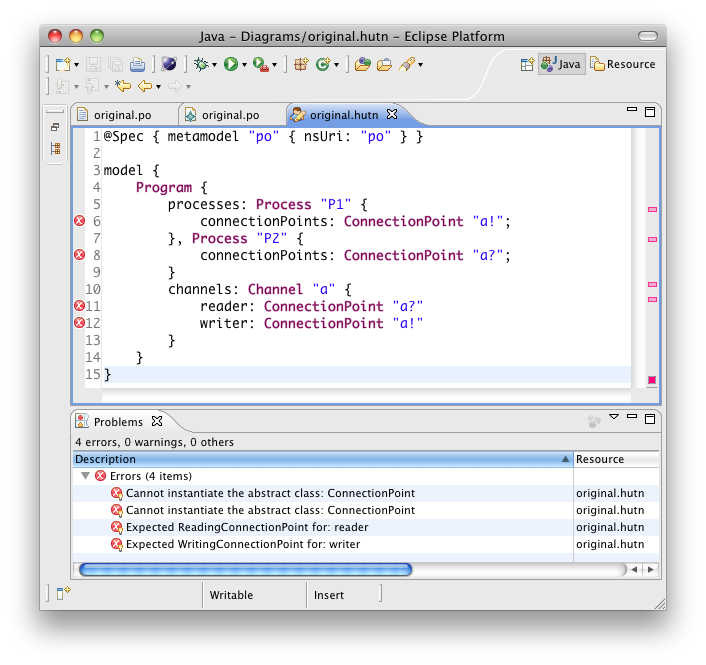
\includegraphics[width=13.5cm]{6.Evaluation/images/user_driven/po_hutn.png}
  \caption{HUTN source prior to migration}
  \label{fig:po_hutn}
\end{figure}

Conformance problems are reconciled manually by the user, who edits the HUTN source. Conformance is automatically checked whenever the HUTN is changed. For example, Figure~\ref{fig:po_hutn_partial} shows the HUTN editor when migration is partially complete. Some of the conformance problems have been reconciled, and the associated error-markers are no longer displayed in the left-hand margin.

\begin{figure}[htbp]
  \centering
  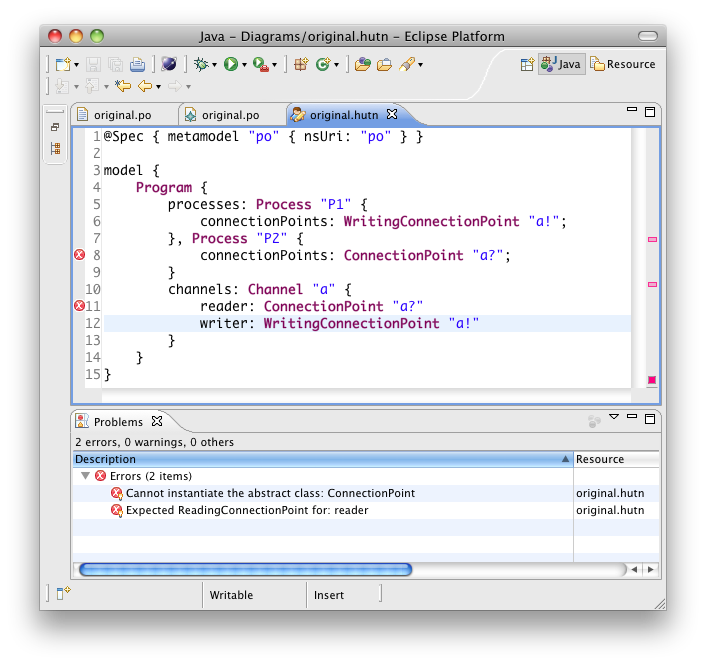
\includegraphics[width=13.5cm]{6.Evaluation/images/user_driven/po_hutn_partial.png}
  \caption{HUTN source part way through migration}
  \label{fig:po_hutn_partial}
\end{figure}

When no conformance errors remain, Epsilon HUTN automatically generates XMI for reconciled model, and the user can now successfully load the migrated model with the graphical editor.

\subsection{Comparison}
\label{subsec:user_driven_example_comparison}
To suggest ways in which dedicated structures for user-driven co-evolution might increase developer productivity, the two user-driven co-evolution approaches demonstrated above are now compared. The first approach, described in Section~\ref{subsec:user-driven_co-evolution_with_emf}, uses only those tools available in EMF for performing user-driven co-evolution, while the second approach, described in Section~\ref{subsec:user-driven_co-evolution_with_dedicated_structures} uses two of the structures introduced in Chapter~\ref{Implementation}. Applying the approaches to the process-oriented example highlighted differences between the modelling notations used, and the way in which conformance problems were reported.

\subsubsection{Differences in modelling notation}
For reconciling conformance problems, the two approaches used different modelling notations, XMI and Epsilon HUTN. Differences in notation that might influence developer productivity during user-driven co-evolution are now discussed. However, further work is required to more rigorously explore the extent to which developer productivity is affected by the modelling notation, as discussed in Section~\ref{subsec:user_driven_further_work}.

The way in which the type of a model element is specified is different in XMI and HUTN. In XMI, type information can be omitted in some circumstances, but must be included in others. In HUTN, type information is mandatory for every model element. Consequently, every HUTN document contains examples of how type information should be specified, whereas XMI documents may not. 

Reference values are specified using paths in XMI (such as \texttt{//@pro\-ces\-ses.1/@con\-nec\-ti\-onPo\-in\-ts.0}) and by name (such as \texttt{a?}) in HUTN. XMI paths are constructed in terms of a document's structure and, as such, rely on implementation details. The name of a model element, on the other hand, is specified in the model, and does not rely on any implementation details. Consequently, it is conceivable that fewer mistakes will be made during user-driven co-evolution when reference values are specified by name rather than with the structural details of a model.

\subsubsection{Differences in conformance reports}
The two approaches differ in the way in which conformance problems were reported, and, as a consequence, the first approach was iterative and the second was not. The differences might influence developer productivity during user-driven co-evolution. Again, further work is required to rigorously explore the extent to which developer productivity is affected by the differences in conformance reporting, as discussed in Section~\ref{subsec:user_driven_further_work}.

With EMF, user-driven co-evolution is an iterative process. Conformance errors are fixed by the user, who then reloads the reconciled model (with, for example, a graphical editor). Each time the model is loaded, further conformance problems might be reported when, for example, the user makes a mistake when reconciling the model. By contrast, the implementation of HUTN described in Section~\ref{sec:notation} uses a background compiler that checks conformance while the user edits the HUTN source. When the user makes a mistake reconciling the HUTN source, the error is reported immediately, and does not require the model to be loaded in the graphical editor.

Although not demonstrated in the process-oriented example, user-driven co-evolution would, for some types of metamodel changes, remain an iterative process even if EMF performed conformance checking in the background. Because EMF uses a multi-pass parser, some types of conformance problem are reported before other types. For example, conformance problems relating to multiplicity constraints (e.g. a process does not specify a name, but name is a mandatory attribute) are reported after all other types of conformance problem. When several types of conformance problem have been affected by metamodel changes, user-driven co-evolution with EMF would remain an iterative process. Single-pass, background parsing is required to display all conformance problems while the user migrates a model.

\subsection{Towards a more thorough comparison}
\label{subsec:user_driven_further_work}
Extensions to the evaluation of user-driven co-evolution are now discussed. In particular, alternative comparison methods might enable a more rigorous exploration of the ways in which dedicated structures for performing user-driven co-evolution influence developer productivity.

A comprehensive user study, involving hundreds of users, is one means for exploring the extent to which productivity varies when dedicated structures are used to perform user-driven co-evolution. Ideally, participants for the study would constitute a large and representative sample of the users of EMF. Productivity might be measured by the time taken to perform co-evolution. To remove a potential source of bias, several examples of co-evolution might be used.

% Autocompletion
% Iterative problem reporting might be good - perhaps it could be used to show "likely" root cause problems first, and problems less likely to be a root cause later?s
% Other types of XMI ID: UUID, derived


Locating a reasonable number of participants and co-evolution examples for a comprehensive user study was not feasible in the context of this thesis. Nevertheless, the comparison presented in Section~\ref{subsec:user_driven_example_comparison} suggests that productivity might be increased when using dedicated structures for user-driven co-evolution. By demonstrating an approach to user-driven co-evolution that uses dedicated structures, this thesis provides a foundation for further, more rigorous evaluation. For example, the HUTN specification \cite{hutn} makes claims about the human-usability of the notation, but the usability of HUTN has not been studied or compared with other modelling notations. Epsilon HUTN (Section~\ref{sec:notation}) is a reference implementation of HUTN and, as demonstrated by the evaluation presented here, facilitates the evaluation of HUTN and the comparison of HUTN to other modelling notations, such as XMI.


\subsection{Summary}
\label{subsec:user_driven_example_summary}
This section has demonstrated two approaches to user-driven co-evolution using a co-evolution example from a project in which a graphical model editor was created for process-oriented programs. The first approach used the structures available in EMF alone, while the second approach used two of the structures described in Chapter~\ref{Implementation}. Comparing the two approaches highlighted differences between the way in which conformance problems were reported and between the modelling notations used to reconcile conformance problems. The comparison described in Section~\ref{subsec:user_driven_example_comparison} suggests that developer productivity might be increased by using the second approach, but, as discussed in Section~\ref{subsec:user_driven_further_work}, further work is required to more rigorously evaluate this claim.


%!TEX root = /Users/louis/Documents/PhD/Deliverables/Thesis/thesis.tex

\subsection{Quantitive Comparison of Model Migration Languages}
In Section~\ref{subsec:requirements_identification}, the following research requirement was identified: \emph{This thesis must implement and evaluate a domain-specific language for specifying and executing model migration strategies, comparing it to existing languages for specifying model migration strategies.} As discussed in Section~\ref{subsec:flock_implementation}, this thesis contributes Epsilon Flock, a domain-specific language for model migration. This section fulfils the second part of the above research requirement, comparing Flock with languages that are used in contemporary migration tools. 

In developer-driven migration, a programming language codifies the migration strategy. Because migration involves deriving the migrated model from the original, migration strategies typically access information from the original model and, based on that information, update the migrated model in some way. As such, migration is written in a language with constructs for accessing and updating the original and migrated models. Here, those language constructs are termed \textit{model operations}. Using examples of co-evolution, this section explores the variation in frequency of \emph{model operation} over different model migration languages, and discusses to what extent the results of this comparison can be used to assess the suitability of the languages considered for model migration.

As discussed in Chapter~\ref{Implementation}, the languages currently used for model migration vary. Model-to-model transformation languages are used in some migration tools (e.g. \cite{cicchetti,garces}); general-purpose languages in others (e.g. \cite{ecore2ecore,cope}). Irrespective of the language used for migration, the way in which a migration tool relates original and migrated model elements falls into one of two categories: new- or existing-target, which were first introduced in Section~\ref{subsec:existing_migration_languages}. In the former, the migrated model is created afresh by the execution of the migration strategy. In the latter, the migrated model is initialised as a copy of the original model and then the migration strategy is executed.

Flock contributes a novel approach for relating original and migrated model elements, termed conservative copy. Conservative copy is a hybrid of new- and existing-target approaches. This section compares new-target, existing-target and conservative copy in the context of model migration. \footnote{TODO: Explain the structure of the rest of this section}

\subsubsection{Data}
Five examples of co-evolution were used to compare new-target, existing-target and conservative copy. This section briefly discusses the data used in the comparison.

\paragraph{Co-evolution Examples}
TODO: GMFx2, Newsgroupsx2, UML Activities. Briefly describe these and explain where they came from.

These examples were not used in the work described in Chapters~\ref{Analysis} and \ref{Implementation}.

\pargraph{Selection of Migration Languages}
As discussed above, there are two ways in which existing migration languages relate original and migrated model elements, new- and existing-target. Flock contributes a third way, conservative copy. For the comparison with Flock, one new- and one existing-target language was chosen.

The Atlas Transformation Language (ATL), a model-to-model transformation language has been used in \cite{cicchetti,garces} for model migration. As discussed in Section~\ref{subsec:existing_migration_languages}, model-to-model transformation languages support only new-target transformations for model migration\foonote{Because, in model migration, the source and target metamodels are not the same.}.

The author is aware of two approaches to migration that use existing-target transformations. In COPE \cite{cope}, migration strategies are hand-written in Groovy when no co-evolutionary operator can be applied. As discussed in Section~\ref{subsec:existing_migration_languages}, COPE's Groovy migration strategies use an existing-target approach. COPE provides 6\footnote{check this} operations for interacting with model elements, such as \texttt{set}, for changing the value of a feature, and \texttt{unset}, for removing all values from a feature. In the remainder of this section, the term \emph{Groovy-for-COPE} is used to refer to the combination of the Groovy programming language and the operators provided by COPE for use in hand-written migration strategies. In Ecore2Ecore \cite{ecore2ecore}, migration is performed when the original model is loaded, effectively an existing-target approach. Ecore2Ecore migration strategies are written in Java and must interact with libraries for interacting with EMF and XML.

The comparison to Flock described in this section uses ATL to represent new-target approaches and Groovy-for-COPE to represent existing-target approaches. Groovy-for-COPE was preferred to Ecore2Ecore because the latter is not as expressive\foonote{Communication with Ed Merks, Eclipse Modeling Project leader, 2009, available at \url{http://www.eclipse.org/forums/index.php?t=tree&goto=486690&S=b1fdb2853760c9ce6b6b48d3a01b9aac}} and cannot be used for migration in the co-evolution examples considered in this section.

\subsubsection{Method}
For each example of co-evolution, a migration strategy was written using each migration language (namely ATL, Groovy-for-COPE and Flock). The correctness of the migration strategy was assured by comparing the migrated models provided by the co-evolution example with the result of executing the migration strategy on the original models provided by the co-evolution example.

For each migration language, a set of model operations were identified, as described in Section~\ref{subsec:model_migration_languages}. A program was written to count the number of \emph{model operations} appearing in each migration strategy. The counting program was tested by writing migration strategies in each language for the co-evolution examples identified in Chapter~\ref{Analysis}.

There is one non-trivial threat to the validity of the comparison performed in this section. The author wrote the migration strategies for Flock (a migration language that the author developed) and for the other migration languages considered (which the author has not developed). Therefore, it is possible that the migration strategies written in the latter may contain more model operations than necessary. In some cases, it was possible to reduce the effects of this threat by re-using or adapting existing migration strategy code written by the migration language authors. This is discussed further in Section~\ref{model_migration_languages}.


\subsubsection{Model Migration Languages}
\label{subsec:model_migration_languages}
The variation in frequency of model operations was explored across three model migration languages, ATL, Groovy-for-COPE and Flock. Here, the model operations of each language are identified. In addition, the extent to which the comparison described in this section was able to use code written by the authors of each language is discussed.


\paragraph{Atlas Transformation Language}
The Atlas Transformation Language (ATL), ....

TODO: Delete isn't measure because elements aren't deleted, they're simply not copied.
TODO: Where do COPE / FLock use new? Why doesn't ATL? If it does, I need to count those too. OR, reconsider counting new - is it necessary?

\begin{itemize}
	\item Assignment to a feature:
	\subitem \texttt{<element>.<feature> <- <value>} 
	
	\item Changing the type of a model element:
	\subitem \texttt{rule \{ from <name> : <original_type> to <name> : <migrated_type> \}}
\end{itemize}

The \texttt{to} part of a \texttt{migrate} rule is optional. \texttt{Migrate} rules without \texttt{to} parts were not counted as model operations.

\paragraph{Groovy-for-COPE}
In COPE \cite{cope}, migration strategies are codified in Groovy, a general-purpose, dynamically-typed programming language. COPE provides model operations for manipulating the migrated model via a metamodel-independent representation, as discussed in Chapters~\ref{Analysis} and \ref{Implementation}. For Groovy-for-COPE, the following model operations were counted:

\begin{itemize}
	\item Assignment to a feature:
	\subitem \texttt{<element>.<feature> = <value>}
	\subitem \texttt{<element>.<feature>.add(<value>)}
	\subitem \texttt{<element>.<feature>.addAll(<collection\_of\_values>)}
	\subitem \texttt{<element>.set(<feature>) = <value>}
	
	\item Unsetting a feature:
	\subitem \texttt{<element>.<feature>.unset()}	
	
	\item Creating a new model element:
	\subitem \texttt{<element\_type>.newInstance()}
	
	\item Deleting a model element:
	\subitem \texttt{delete <element>}
	
	\item Changing the type of a model element:
	\subitem \texttt{<element>.migrate(<element\_type>)}
\end{itemize}

COPE provides a library of built-in, reusable co-evolutionary operators. Each co-evolutionary operator specifies a metamodel evolution along with a corresponding model migration strategy. For example, the ``Make Reference Containment'' operator evolves the metamodel such that a non-containment reference becomes a containment reference and migrates models such that the values of the evolved reference are replaced by copies.

As such, writing the Groovy migration strategy for the examples of co-evolution considered in this section involved, where possible, applying an appropriate COPE co-evolutionary operator and counting the number of model operations in the generated migration strategy. Not all examples could be completely specified using COPE co-evolutionary operator. In these cases, the Groovy migration strategy was written by the author.


\paragraph{Epsilon Flock}
Epsilon Flock, a transformation language tailored for model migration, was developed in this thesis and discussed in Chapter~\ref{Implementation}. Flock uses the Epsilon Object Language (EOL) \cite{kolovos06eol} to access and update model values. In addition, Flock defines \texttt{migrate} rules, which can be used to change the type of a model element. For Flock, the following model operations were counted:

\begin{itemize}
	\item Assignment to a feature:
	\subitem \texttt{<element>.<feature> := <value>} 
	\subitem \texttt{<element>.<feature>.add(<value>)}
	\subitem \texttt{<element>.<feature>.addAll(<collection\_of\_values>)}

	\item Creating a new model element:
	\subitem \texttt{new <element\_type>}
	
	\item Deleting a model element:
	\subitem \texttt{delete <element>}
	
	\item Changing the type of a model element:
	\subitem \texttt{migrate <original_type> to <migrated_type>}
\end{itemize}

The \texttt{to} part of a \texttt{migrate} rule is optional. \texttt{Migrate} rules without \texttt{to} parts were not counted as model operations.


\subsubsection{Results}
\label{subsec:quantitive_results}
By measuring the number of model operations in model migration strategies, the way in which each co-evolution approach relates original and migrated model elements was investigated. Five examples of model migration were measured to obtain the results shown in Table~\ref{tab:model_operations_results}. 

\begin{table}
	\caption{Model operation frequency. An asterisk denotes an example that is not supported by Ecore2Ecore.}
	\centering
	\begin{tabular}{|r|c|c|c|}
		\hline
		Name                        & ATL & COPE & Flock \\
		\hline
		\hline
		Newsgroup Extract Person    & 9  &  7  &  6  \\
		\hline                       
		Newsgroup Resolve Replies   &  8  &  3  &  2  \\
		\hline                       
		UML Activity Diagrams       &  26  &  TBC  &  17  \\
		\hline                       
		GMF Graph                   &  101  &  TBC  &  16  \\
		\hline                       
		GMF Gen2009                 &  310  &  TBC  &  21  \\
		\hline
		\hline
		Totals                       & TBC & TBC  &  TBC \\
		\hline
		Averages                     &  TBC  &  TBC  &  TBC \\
		\hline
	\end{tabular}
	\label{tab:model_operations_results}
\end{table}

TODO: might be interesting to reinstate the table for results from examples described in analysis chapter.

TODO: Comment on why GMF results are so much higher for ATL (It's because the source metamodels contain a lot of features. The UML example would have had similar differences in figures, but uses a minimal metamodel because ATL / COPE don't support MDR).

The results in Table~\ref{tab:model_operations_results} show that no migration strategy encoded in Flock contained less model operations when encoded in Groovy-for-COPE or ATL. For the majority of examples, no migration strategy encoded in Groovy-for-COPE contained less model operations when encoded in ETL. The reasons for the results shown in Table~\ref{tab:model_operations_results} are now investigated.

\paragrah{Copying Strategy}
Each approach initialises the migrated model in a different way: ATL initialises an empty model, while COPE initialises a complete copy of the original model. Flock initialises the migrated model by copying only those model elements from the original model that conform to the migrated metamodel. The effects of these different copying strategies can be seen in many of the examples in Table~\ref{tab:model_operations_results}. To explain this, a smaller example of co-evolution is used below.

A Petri \texttt{Net} comprises \texttt{Place}s and \texttt{Transition}s (Figure~\ref{fig:original_mm}). A \texttt{Place} has any number of \texttt{src} or \texttt{dst} \texttt{Transition}s. Similarly, a \texttt{Transition} has at least one \texttt{src} and \texttt{dst} \texttt{Place}. The metamodel in Figure~\ref{fig:original_mm} is to be evolved so as to support weighted connections between \texttt{Place}s and \texttt{Transition}s and between \texttt{Transition}s and \texttt{Place}s.

\begin{figure}[htbp]
  \centering
  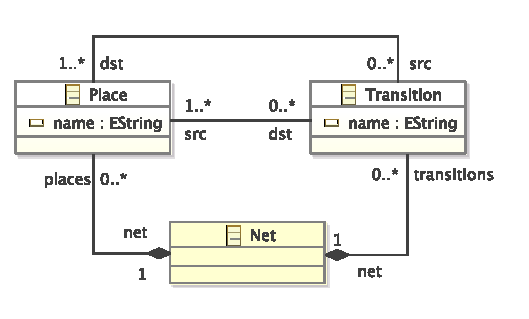
\includegraphics[scale=0.75]{petri_nets_step0.pdf}
  \caption{Original Petri nets metamodel.}
  \label{fig:original_mm}
\end{figure}

The evolved metamodel is shown in Figure~\ref{fig:evolved_mm}. \texttt{Place}s are connected to \texttt{Transition}s via instances of \texttt{PTArc}. Likewise, \texttt{Transition}s are connected to \texttt{Place}s via \texttt{TPArc}. Both \texttt{PTArc} and \texttt{TPArc} inherit from \texttt{Arc}, and therefore can be used to specify a \texttt{weight}.

\begin{figure}[htbp]
  \centering
  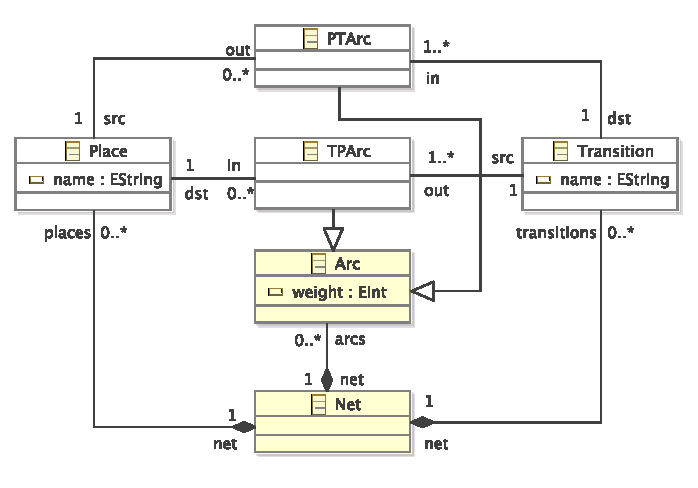
\includegraphics[scale=0.75]{petri_nets_step1.pdf}
  \caption{Evolved Petri nets metamodel.}
  \label{fig:evolved_mm}
\end{figure}

Models that were consistent with the original metamodel may not be consistent with the evolved metamodel. For example, \texttt{Transition} objects can no longer define values for \texttt{src} and \texttt{dst} features, and must define at least one value for the \texttt{in} and \texttt{out} features.

The migration strategy for this evolution varies when specified in ATL, Groovy-for-COPE and Flock, largely due to the differences in the way in which each approach initialises migrated models. When specified in ATL, migration must copy values from original to migrated model, as shown on lines 5-6, 12 and 20 of Listing~\ref{lst:quantitive_etl}. When using Groovy-for-COPE, values contained in slots that no longer correspond to features in the migrated metamodel must be unset, as shown on lines 2, 9 and 18-19 of Listing~\ref{lst:quantitive_cope}. Finally, Flock initialises the migrated model by copying values only for those features that remain unchanged in the migrated model. Consequently, no explicit copying or unsetting is required in Listing~\ref{lst:quantitive_flock}; the migration strategy manipulates only metafeatures that do not exist in the evolved metamodel (\texttt{Transition\#src} and \texttt{Transition\#dst}) and the new metaclasses, \texttt{TPArc} and \texttt{PTArc}.

\begin{lstlisting}[basicstyle=\ttfamily\footnotesize, flexiblecolumns=true, numbers=left, nolol=true, caption=Petri nets model migration in ATL, label=lst:quantitive_etl, language=ETL, tabsize=2]
rule Nets {
	from
		o : Before!Net
	to
	  m : After!Net ( places <- o.places, transitions <- o.transitions )
}

rule Places {
	from
		o : Before!Place
	to
		m : After!Place ( name <- o.name )
}

rule Transitions {
	from
		o : Before!Transition
	to
		m : After!Transition (
			name <- o.name,
			"in" <- o.src->collect(p | thisModule.PTArcs(p,o)),
			out  <- o.dst->collect(p | thisModule.TPArcs(o,p))
		)
}

lazy rule PTArcs {
	from
		place       : Before!Place,
		destination : Before!Transition
	to
		ptarcs : After!PTArc (
			src <- place,
			dst <- destination,
			net <- destination.net
		)
}

lazy rule TPArcs {
	from
		transition  : Before!Transition,
		destination : Before!Place
	to
		tparcs : After!TPArc (
			src <- transition,
			dst <- destination,
			net <- transition.net
		)
}
\end{lstlisting}


\begin{lstlisting}[basicstyle=\ttfamily\footnotesize, flexiblecolumns=true, numbers=left, nolol=true, caption=Petri nets model migration in COPE, label=lst:quantitive_cope, language=Java, tabsize=2]
for (transition in Transition.allInstances) {
  for (source in transition.unset('src')) {
    def arc = petrinets.PTArc.newInstance()
    arc.src = source
    arc.dst = transition
    arc.net = transition.net
  }

  for (destination in transition.unset('dst')) {
    def arc = petrinets.TPArc.newInstance() 
    arc.src = transition
    arc.dst = destination
    arc.net = transition.net
  }
}

for (place in Place.allInstances) {
  place.unset('src')
  place.unset('dst')
}
\end{lstlisting}


\begin{lstlisting}[basicstyle=\ttfamily\footnotesize, flexiblecolumns=true, numbers=left, nolol=true, caption=Petri nets model migration in Flock, label=lst:quantitive_flock, language=Flock, tabsize=2]
migrate Transition {
  for (source in original.src) {
    var arc := new Migrated!PTArc;
    arc.src := source.equivalent();
    arc.dst := migrated;
    arc.net := original.net.equivalent();
  }

  for (destination in original.dst) {
    var arc := new Migrated!TPArc;
    arc.src := migrated;
    arc.dst := destination.equivalent();
    arc.net := original.net.equivalent();
  }
}
\end{lstlisting}

With regard to the way in which they initialise the migrated model, COPE and ATL are opposites. The former initialises an exact copy of the original model, and so unset operations must be used when the value of a feature should not have been copied. By contrast, the latter initialises an empty model, and so explicit assignment operations must be used to copy values from original to migrated model for each feature that is not affected by the metamodel evolution.

This difference explains the results shown in Table~\ref{tab:model_operations_results}. Firstly, because Flock requires no unsetting of affected model elements nor explicit copying of unaffected model elements, less model operations are used when specifying a migration strategy with Flock than is used when specifying the same migration strategy with Groovy-for-COPE or with ATL. Secondly, there are more features unaffected by metamodel evolution than affected. Consequently, specifying model migration with ATL for the examples shown in Table~\ref{tab:model_operations_results} requires more model operations than in Groovy-for-COPE.


\paragrah{Side-Effects during Initialisation}
The measurements observed for one of the examples of co-evolution from Chapter~\ref{Analysis}, Change Reference to Containment, cannot be explained by the difference in copying strategy. Instead, the way in which models are initialised by the migration languages must be considered. When a reference feature is changed to a containment reference during metamodel evolution, constructing the migrated model by starting from the original model (as is the case with Groovy-for-COPE and, when the feature is not renamed, also Flock) can have side-effects which complicate migration.

In the Change Reference to Containment example, a \texttt{System} initially comprises \texttt{Port}s and \texttt{Signature}s (Figure~\ref{fig:ref2cont_original_mm}). A \texttt{Signature} references any number of \texttt{ports}. The metamodel is to be evolved so that \texttt{Port}s can no longer be shared between \texttt{Signature}s.

\begin{figure}[htbp]
  \centering
  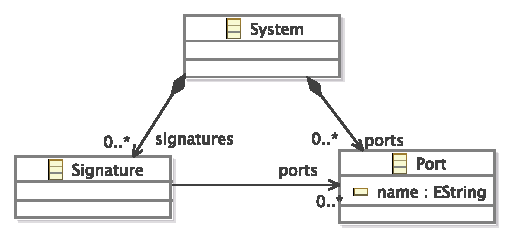
\includegraphics[scale=0.75]{change_ref_to_cont_before.pdf}
  \caption{Original metamodel.}
  \label{fig:ref2cont_original_mm}
\end{figure}

The evolved metamodel is shown in Figure~\ref{fig:ref2cont_evolved_mm}. \texttt{Signature}s now contain - rather than reference - \texttt{Port}s. Consequently, the \texttt{ports} feature of \texttt{System} is no longer required and is removed.

\begin{figure}[htbp]
  \centering
  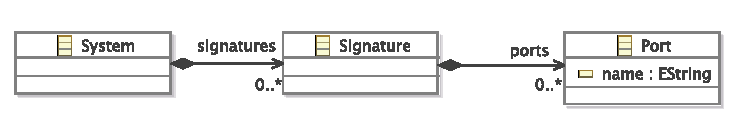
\includegraphics[scale=0.75]{change_ref_to_cont_after.pdf}
  \caption{Evolved metamodel.}
  \label{fig:ref2cont_evolved_mm}
\end{figure}

The migration strategy is straightforward in ATL: for each \texttt{Signature} in the original model, each member of the \texttt{ports} feature is cloned, using a lazy rule, and added to the \texttt{ports} feature of the equivalent \texttt{Signature}.

\begin{lstlisting}[basicstyle=\ttfamily\footnotesize, flexiblecolumns=true, numbers=left, nolol=true, caption=Change R to C model migration in ATL, label=lst:ref2cont_atl, language=ATL, tabsize=2]
rule Systems {
	from
		o : Before!System
	to
		m : After!System ( signatures <- o.signatures )
}

rule Signature {
	from
		o : Before!Signature
	to
		m : After!Signature (
			ports <- o.ports->collect(p | thisModule.Port(p))
		)
}

lazy rule Port {
	from
		o : Before!Port
	to
		m : After!Port ( name <- o.name )
\end{lstlisting}

In Flock and Groovy-for-COPE, migration is less straightforward because, during migration, the value of a containment reference (\texttt{Signature\#ports}) is set automatically by the migration strategy execution engine. When a containment reference is set, the contained objects are removed from their previous containment reference (i.e. setting a containment reference can have side-effects). Therefore, in a \texttt{System} where more than one \texttt{Signature} references the same \texttt{Port}, the migrated model cannot be formed by copying the contents of \texttt{Signature\#ports} from the original model. Attempting to do so causes each \texttt{Port} to be contained only in the last referencing \texttt{Signature} that was copied.

In Groovy-for-COPE, the containment nature of the reference is not enforced until after the migration strategy is executed. Hence, the migration strategy can be specified by unsetting the contents of the \texttt{ports} reference (line 4 of Listing~\ref{lst:ref2cont_cope}), and creating a copy of each referenced \texttt{Port} (lines 5-7 of Listing~\ref{lst:ref2cont_cope}). Unlike the ATL migration strategy, the ports in the Groovy-for-COPE migration strategy are cloned in the same model as the original port. Consequently, the Groovy-for-COPE migration strategy must either only clone ports that are referenced by more than one signature or clone every referenced port, but delete all of the original ports. The latter approach requires 2 more model operations (to populate and delete the original ports) than the former (shown in Listing~\ref{lst:ref2cont_cope}).

\begin{lstlisting}[basicstyle=\ttfamily\footnotesize, flexiblecolumns=true, numbers=left, nolol=true, caption=Change R to C model migration in COPE, label=lst:ref2cont_cope, language=COPE, tabsize=2]
def contained = []

for(signature in refactorings_changeRefToCont.Signature.allInstances) {
  for(port in signature.ports)) {
	  // when more than one Signature references this port
	  if (contained.contains(port)) {
      def clone = Port.newInstance()
      clone.name = port.name
      signature.ports.add(clone)
      signature.ports.remove(port)
		} else {
			contained.add(port)
		}
  }
}

for(port in refactorings_changeRefToCont.Port.allInstances) {
	if (not refactorings_changeRefToCont.Signature.allInstances.any { it.ports.contains(port) }) {
	  	port.delete()
	}
}
\end{lstlisting}

In Flock, the containment nature of the reference is enforced when the migrated model is initialised. Because changing the contents of a containment reference can have side-effects, a \texttt{Port} that appears in the \texttt{ports} reference of a \texttt{Signature} in the original model may not have been automatically copied to the \texttt{ports} reference of the equivalent \texttt{Signature} in the migrated model during initialisation. Consequently, the migration strategy must check the \texttt{ports} reference of each migrated \texttt{Signature}, cloning only those \texttt{Port}s that have not be automatically copied during initialisation (see line 3 of Listing~\ref{lst:ref2cont_flock}).

\begin{lstlisting}[basicstyle=\ttfamily\footnotesize, flexiblecolumns=true, numbers=left, nolol=true, caption=Change R to C model migration in Flock, label=lst:ref2cont_flock, language=Flock, tabsize=2]
migrate Signature {
	for (port in original.ports) {
		if (migrated.ports.excludes(port.equivalent())) {
			var clone := new Migrated!Port;
			clone.name := port.name;
			migrated.ports.add(clone);
		}
	}
}

delete Port when: not Original!Signature.all.exists(s|s.ports.includes(original))
\end{lstlisting}


The Groovy-for-COPE and Flock migration strategies must also remove any \texttt{Port}s which are not referenced by any \texttt{Signature} (lines 17-21 of Listing~\ref{lst:ref2cont_cope}, and line 11 of Listing~\ref{lst:ref2cont_flock} respectively), whereas the ATL migration strategy, which initialises any empty migrated model, does not copy unreferenced \texttt{Port}s.

When a non-containment reference is changed to a containment reference, a Flock migration strategy requires one more more model operation than the equivalent ATL migration strategy: to delete model elements that are not contained in any instance of the containment reference (line 11 of Listing~\ref{lst:ref2cont_flock}). A Groovy-for-COPE migration strategy requires three more model operations than the equivalent ATL migration strategy: one to delete model elements that are not contained in any instance of the containment reference (lines 17-21 of Listing~\ref{lst:ref2cont_cope}), one to dereference model elements that have already been cloned (line 10 of Listing~\ref{lst:ref2cont_cope}), and one to mark a model element as contained (line 12 of Listing~\ref{lst:ref2cont_cope}).  In the example considered here, the ATL migration strategy requires one more model operation than the Flock and Groovy-for-COPE migration strategies (to copy the contents of System\#signature features from original to migrated model), due to the difference in copying strategy. This leads to the result shown in Table~\ref{tab:model_operations_results}: the Flock and ATL migration strategies have an equal number of model operations, while the COPE migration strategy has two more.


\subsubsection{Summary}
This section has compared the model migration languages

- Make clear the contribution: no other research has attempted to compare model migration languages. It's not clear how it should be done. This is a start. 
- Not trying to argue that the figures are statistically significant. Just an approximation of what we're trying to measure.
- Extensions: measure cyclomatic complexity, etc

%!TEX root = /Users/louis/Documents/PhD/Deliverables/Thesis/thesis.tex

\section[Evaluating Epsilon Flock and other Co-evolution Tools][Evaluating Flock and other Co-evolution Tools]{Evaluating Epsilon Flock and other Co-evolution Tools}
\label{sec:collaborative_comparison}
This section assesses the extent to which Epsilon Flock (Section~\ref{sec:flock}) can be used for automating developer-driven co-evolution. To this end, Flock is compared to three co-evolution tools using an expert evaluation. While Chapter~\ref{Analysis} highlighted theoretical differences between co-evolution tools, the expert evaluation explored the ways in which migration tools compare in practice.

One aspect of Flock, conciseness, was evaluated in Section~\ref{sec:quantitive}. The evaluation performed in this section evaluates several further aspects of model migration tools. The results of the comparison, described in Section~\ref{sec:discussion}, suggest situations in which using Flock leads to increased productivity of model migration, and, conversely, situations in which the other co-evolution tools provide benefits over using Flock. Additionally, the expert evaluation aimed to  simplify the selection of migration tools by recommending tools for particular situations or requirements. Tool selection advice was synthesised from the expert evaluation, and recommends tools that are suitable, for example, when scalability is a concern (many large models are to be migrated).

The way in which Flock affects the productivity of model migration might have been explored using a comprehensive user-study, involving hundreds of users. However, locating a large number of participants with expertise in model-driven engineering was not possible given the time constraints of the research. Alternatively, Flock and several further co-evolution tools might have been applied, by the author, to a large, independent co-evolution example in a case study. However, exploring the variations in productivity of the co-evolution tools would likely have been challenging as the author is obviously more familiar with Flock than the other tools. Instead, the comparison of co-evolution tools was performed using an expert evaluation.

The remainder of this section describes the comparison method, reports results and tool selection guidance, and discusses the situations in which Flock was identified as stronger or weaker than the other co-evolution tools. Section~\ref{sec:method} describes the way in which the co-evolution tools were selected, comparison criteria were identified and the way in which the tools were applied to two co-evolution examples. The experts' experiences with each tool are reported in Section~\ref{sec:results}. Section~\ref{sec:discussion} presents the experts' guidance for identifying the most appropriate model migration tool in different situations, and the section concludes with a description of the strengths and weaknesses of Flock.

\begin{framed}
Section~\ref{sec:collaborative_comparison} is based on joint work with Markus Herrmannsd\"{o}rfer (a research student at Technische Universit\"at M\"unchen), James Williams (a research student in this department), Dimitrios Kolovos (a lecturer in this department) and Kelly Garc\'{e}s (then a research student at EMN-INRIA / LINA-INRIA in Nantes), and has been published in \cite{rose10comparison}. Garc\'{e}s provided assistance with installing and configuration one of the migration tools, and commented on a draft of the paper. Herrmannsd\"{o}rfer, Williams and Kolovos played a larger role in the comparison.
\end{framed}

\subsection{Comparison Method}
\label{sec:method}

\newcommand{\mm}[1]{\texttt{#1}}
The comparison described in this section is based on practical application of the tools to the co-evolution examples described below. This section also discusses the tool selection and comparison processes. Herrmannsd\"{o}rfer and the author identified the co-evolution examples, and formulated the comparison process.

\subsubsection{Co-Evolution Examples}
\label{subsec:method_examples}
To compare migration tools, two examples of co-evolution were used. The first, Petri nets, was first described in Section~\ref{sec:analyis_of_languages_used_for_migration} and is a well-known problem in the model migration literature. The Petri nets example was used to test the installation and configuration of the migration tools. The second, GMF, is a larger example taken from a real-world model-driven development project, and was identified as a potentially useful example for co-evolution case studies in Chapter~\ref{Analysis} and in \cite{herrmannsdoerfer09gmf}.

\paragraph{Petri Nets.}
The first example is the Petri nets example, which was described in Section~\ref{sec:analyis_of_languages_used_for_migration}, and is repeated in Figure~\ref{fig:petri_nets_mms_repeated}. During metamodel evolution, the \mm{PTArc} and \mm{TPArc} classes are introduced to allow the specification of weighted arcs.

\begin{figure}[htbp]
	\centering
	\subfigure[Original metamodel.]
	{
	    \label{fig:petri_nets_original_mm_repeated}
	    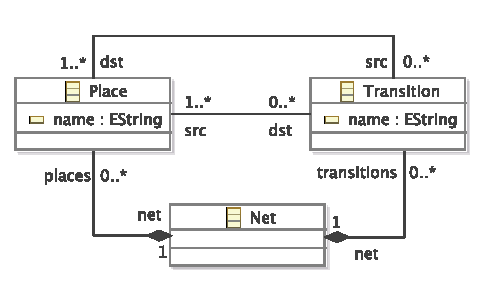
\includegraphics[scale=0.75]{5.Implementation/images/petri_nets_before.pdf}
	}
	\subfigure[Evolved metamodel.]
	{
	    \label{fig:petri_nets_evolved_mm_repeated}
	    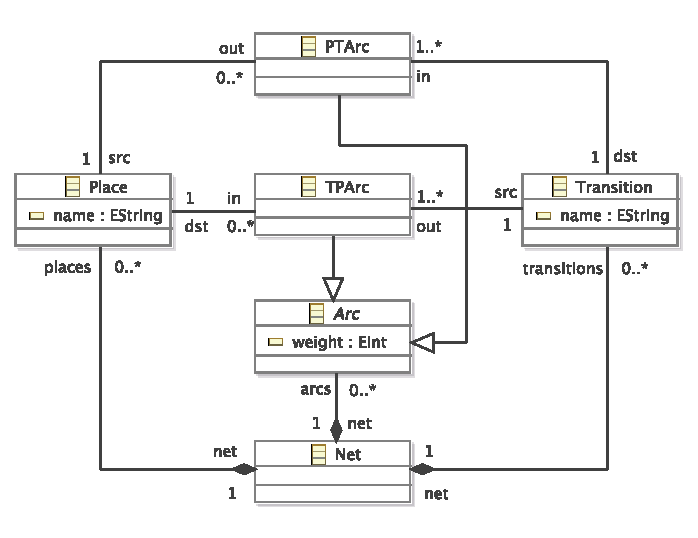
\includegraphics[scale=0.75]{5.Implementation/images/petri_nets_after.pdf}
	}
	\caption[Exemplar metamodel evolution (Petri nets)]{Petri nets metamodel evolution (taken from \cite{rose10flock}, and from Section~\ref{sec:analyis_of_languages_used_for_migration}).}
\label{fig:petri_nets_mms_repeated}
\end{figure}

\paragraph{GMF.}
The second example is taken from GMF \cite{gronback09emp}, an Eclipse project for generating graphical editors for models. The development of GMF is model-driven and utilises four domain-specific metamodels. Here, we consider one of those metamodels, GMF Graph, and its evolution between GMF versions 1.0 and 2.0. The GMF Graph example is now summarised, and more details can be found in Section~\ref{subsec:gmf_graph}.

\begin{figure}[htbp]
	\centering
	\subfigure[Original metamodel.]
	{
	    \label{fig:gmf_graph_mm_original}
	    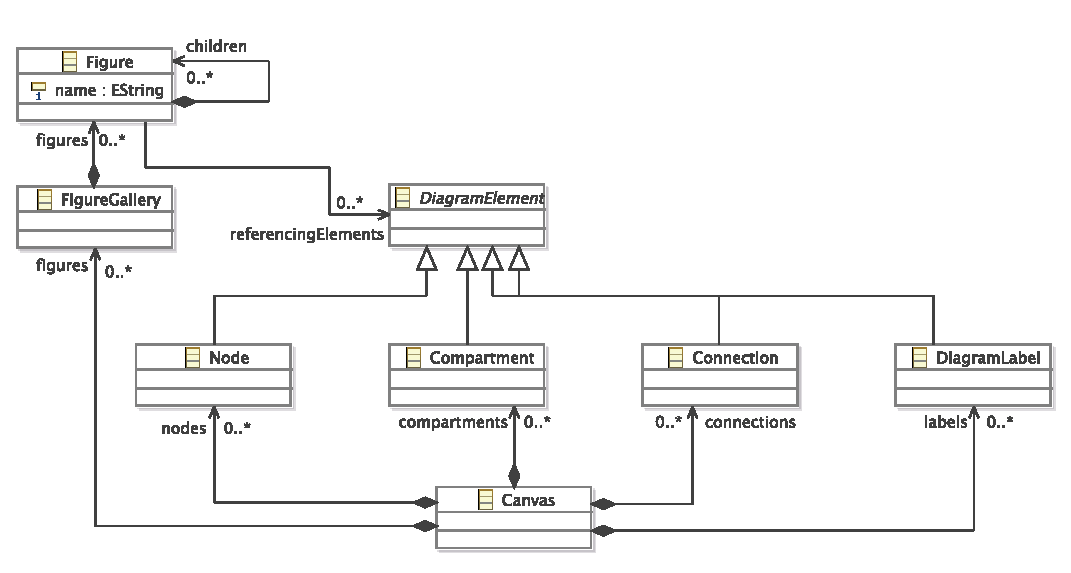
\includegraphics[width=10cm]{A.3.MigrationStrategies/images/gmf/graph_before.pdf}
	}
	\subfigure[Evolved metamodel.]
	{
	    \label{fig:gmf_graph_mm_evolved}
	    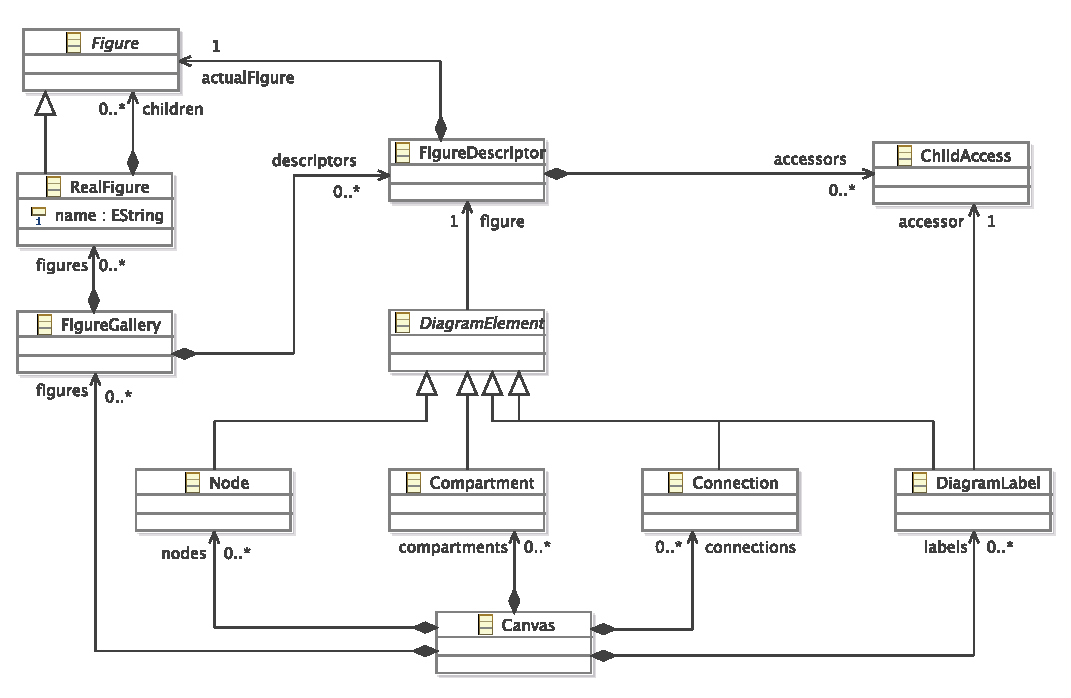
\includegraphics[width=10cm]{A.3.MigrationStrategies/images/gmf/graph_after.pdf}
	}
	\caption{GMF graph metamodel evolution}
\label{fig:gmf_graph_mms}
\end{figure}

The GMF Graph metamodel (Figure~\ref{fig:gmf_graph_mms}) describes the appearance of the generated graphical model editor. As described in the GMF Graph documentation\footnote{\url{http://wiki.eclipse.org/GMFGraph_Hints}}, the Graph metamodel from GMF 1.0 was evolved -- as shown in Figure~\ref{fig:gmf_graph_mm_evolved} -- to facilitate greater re-use of figures by introducing a proxy~\cite{gamma95patterns} for \mm{Fi\-gu\-re}, termed \mm{Fi\-gu\-reDe\-sc\-ri\-pt\-or}. The original \mm{re\-fe\-re\-nc\-in\-gEl\-em\-en\-ts} reference was removed, and an extra metaclass, \mm{Ch\-il\-dAc\-ce\-ss} in its place. Section~\ref{subsec:gmf_graph} discusses the metamodel changes in more detail.

GMF provides a migrating algorithm that produces a model conforming to the evolved Graph metamodel from a model conforming to the original Graph metamodel. In GMF, migration is implemented using Java. The GMF source code includes two example editors, for which the source code management system contains versions conforming to GMF 1.0 and GMF 2.0. For the comparison of migration tools described in this paper, the migrating algorithm and example editors provided by GMF were used to determine the correctness of the migration strategies produced by using each model migration tool.

\subsubsection{Compared Tools}
\label{subsec:method_tools}
The expert evaluation compares Flock (a manual specification tool), COPE (an operator-based tool) and AML (an inference tool). A further tool from the manual specification category, Ecore2Ecore, was included because it is distributed with the Eclipse Modeling Framework (EMF), arguably the most widely used modelling framework. AML, COPE and Ecore2Ecore were discussed in Chapter~\ref{Analysis}, and Flock in Chapter~\ref{Implementation}.


\subsubsection{Comparison Process}
\label{subsec:method_process}
The comparison of migration tools was conducted by applying each of the four tools (Ecore2Ecore, AML, COPE and Flock) to the two examples of co-evolution (Petri nets and GMF). The developers of each tool were invited to participate in the comparison. The authors of COPE and Flock were able to participate fully, while the authors of Ecore2Ecore and AML were available for guidance, advice, and to comment on preliminary results.

Each tool developer was assigned a migration tool to apply to the two co-evolution examples. Because the authors of Ecore2Ecore and AML could not participate fully in the comparison, two colleagues experienced in model transformation and migration, James Williams and Dimitrios Kolovos, took part. To improve the validity of the comparison, each tool was used by someone other than its developer.

The comparison was conducted in three phases. In the first phase, criteria against which the tools would be compared were identified by discussion between the tool developers. In the second phase, co-evolution of Petri nets was used for familiarisation with the migration tools and to assess the suitability of the comparison criteria. In the third phase, the tools were applied to the larger co-evolution (GMF) and results were drawn from the experiences of the tool developers. Table~\ref{tab:criteria} summarises the comparison criteria used, which provide a foundation for future comparisons. The next section presents, for each criterion, observations from applying the migration tools to the co-evolution examples.

\begin{table}[hbtp]
	\centering
	\begin{tabular}{|p{3cm}|p{9cm}|}
	\hline
	\textbf{Name}    & \textbf{Description} \\
	\hline
	Construction     & Ways in which tool supports the development of migration strategies \\
	\hline
	Change           & Ways in which tool supports change to migration strategies \\
	\hline
	Extensibility    & Extent to which user-defined extensions are supported \\
	\hline
	Re-use           & Mechanisms for re-using migration patterns and logic \\
	\hline
	Conciseness      & Size of migration strategies produced with tool \\
	\hline
	Clarity          & Understandability of migration strategies produced with tool \\
	\hline
	Expressiveness   & Extent to which migration problems can be codified with tool \\
	\hline
	Interoperability & Technical dependencies and procedural assumptions of tool \\
	\hline
	Performance      & Time taken to execute migration \\
	\hline
	\end{tabular}
	\label{tab:criteria}
	\caption{Summary of comparison criteria.}
\end{table}


\subsection{Comparison Results}
\label{sec:results}
This section reports the similarities and differences of each tool, using the nine criteria described above. The migration strategies formulated with each tool are available online\footnote{\url{http://github.com/louismrose/migration_comparison}}. 

Each subsection below considers one criterion. This section reports the experiences of the developer to which each tool was allocated. As such, this section contains the work of others. Specifically, Herrmannsd\"{o}rfer described Epsilon Flock, Williams described COPE and Kolovos described Ecore2Ecore. (The author described AML, and introduced each criterion). 

\subsubsection{Constructing the migration strategy}
\label{subsec:constructing}
Facilitating the specification and execution of migration strategies is the primary function of model migration tools. This section reports the process for and challenges faced in constructing migration strategies with each tool.

\paragraph{AML.} An AML user specifies a combination of match heuristics from which AML infers a migrating transformation by comparing original and evolved metamodels. Matching strategies are written in a textual syntax, which AML compiles to produce an executable workflow. The workflow is invoked to generate the migrating transformation, codified in the Atlas Transformation Language (ATL) \cite{jouault05transforming}.
%
Devising correct matching strategies is difficult, as AML lacks documentation that describes the input, output and effects of each heuristic. Papers describing AML (such as \cite{garces09managing}) discuss each heuristic, but mostly in a high-level manner. A semantically invalid combination of heuristics can cause a runtime error, while an incorrect combination results in the generation of an incorrect migration transformation. However, once a matching strategy is specified, it can be re-used for similar cases of metamodel evolution. To devise the matching strategies used in this paper, AML's author provided considerable guidance.

\paragraph{COPE.} A COPE user applies \emph{coupled operations} to the original metamodel to form the evolved metamodel. Each coupled operation specifies a metamodel evolution along with a corresponding fragment of the model migration strategy. A history of applied operations is later used to generate a complete migration strategy.
%
As COPE is meant for co-evolution of models and metamodels, reverse engineering a large metamodel can be difficult. Determining which sequence of operations will produce a correct migration is not always straightforward. To aid the user, COPE allows operations to be undone.
%
To help with the migration process, COPE offers the \emph{Convergence View} which utilises EMF Compare to display the differences between two metamodels. While this was useful, it can, understandably, only provide a list of explicit differences and not the semantics of a metamodel change. Consequently, reverse-engineering a large and unfamiliar metamodel is challenging, and migration for the GMF Graph example could only be completed with considerable guidance from the author of COPE. % For example, it may say that one reference's name and type has changed, but in actual fact a reference class was introduced. This meant that on the larger GMF example, an unfamiliar metamodel, it was difficult to determine exactly what changes needed to be made. Of course, this would be less of a challenge for the author of the metamodel, who has an understanding of how it evolved.

\paragraph{Ecore2Ecore.} In Ecore2Ecore model migration is specified in two steps. In the first step, a graphical mapping editor is used to construct a model that declares basic migrations. In this step only very simple migrations such as class and feature renaming can be declared. In the next step, the developer needs to use Java to specify a customised parser (resource handler, in EMF terminology) that can parse models that conform to the original metamodel and migrate them so that they conform to the new metamodel. This customised parser exploits the basic migration information specified in the first step and delegates any changes that it cannot recognise to a particular Java method in the parser for the developer to handle. Handling such changes is tedious as the developer is only provided with the string contents of the unrecognised features and then needs to use low-level techniques -- such as data-type checking and conversion, string splitting and concatenation -- to address them. Here it is worth mentioning that Ecore2Ecore cannot handle all migration scenarios and is limited to cases where only a certain degree of structural change has been introduced between the original and the evolved metamodel. For cases which Ecore2Ecore cannot handle, developers need to specify a custom parser without any support for automated element copying.

\paragraph{Flock.} In Flock, model migration is specified manually. Flock automatically copies only those model elements which still conform to the evolved metamodel. Hence, the user specifies migration only for model elements which no longer conform to the evolved metamodel.
%
Due to the automatic copying algorithm, an empty Flock migration strategy always yields a model conforming to the evolved metamodel. Consequently, a user typically starts with an empty migration strategy and iteratively refines it to migrate non-conforming elements. However, there is no support to ensure that all non-conforming elements are migrated. In the GMF Graph example, completeness could only be ensured by testing with numerous models.
%
Using this method, a migration strategy can be easily encoded for the Petri net example. For the GMF Graph example whose metamodels are larger, it was more difficult, since there is no tool support for analysing the changes between original and evolved metamodel. %to show how to correctly use the elements of original and evolved metamodel. It is necessary to open editors for both metamodel versions and switch between the strategy editor and these editors back and forth.

\subsubsection{Changing the migration strategy}
Migration strategies can change in at least two ways. Firstly, as a migration strategy is developed, testing might reveal errors which need to be corrected. Secondly, further metamodel changes might require changes to an existing migration strategy.

\paragraph{AML.}  Because AML automatically generates migrating transformations, changing the transformation, for example after discovering an error in the matching strategy, is trivial. To migrate models over several versions of a metamodel at once, the migrating transformations generated by AML can be composed by the user. AML provides no tool support for composing transformations.

\paragraph{COPE.} COPE's undo feature
% operation might be intepreted as coupled operation for COPE, so let's use "undo feature" instead
means that incorrect migrations can be easily fixed. COPE stores a history of \emph{releases} -- a set of operations that has been applied between versions of the metamodel. Because the migration code generated from the release history can migrate models conforming to any previous metamodel release, COPE provides a comprehensive means for chaining migration strategies. 

\paragraph{Ecore2Ecore.} Migrations specified using Ecore2Ecore can be modified via the graphical mapping editor and the Java code in the custom model parser. Therefore, developers can use the features of the Eclipse Java IDE to modify and debug migrations. Ecore2Ecore provides no dedicated tool support for composing migrations.

\paragraph{Flock.} There is comprehensive support in Flock for fixing errors. A migration strategy can easily be re-executed using a launch configuration, and migration errors are linked to the line in the migration strategy that caused the error to occur. If the metamodel is further evolved, the original migration strategy has to be extended, since there is no explicit support to chain migration strategies. The full migration strategy may need to be read to know where to extend it.


\subsubsection{Extensibility}
The fundamental constructs used for specifying migration in COPE and AML (operators and match heuristics, respectively) are extensible. Flock and Ecore2E\-core use a more imperative (than declarative) approach, and as such do not provide extensible constructs.

\paragraph{AML.} An AML user can specify additional matching heuristics. This requires understanding of AML's domain-specific language for manipulating the data structures from which migrating transformations are generated.

\paragraph{COPE} provides the user with a large number of operations. If there is no applicable operation, a COPE user can write their own operations using an in-place transformation language embedded into Groovy\footnote{\url{http://groovy.codehaus.org/}}.


\subsubsection{Re-use}
Each migration tool captures patterns that commonly occur in model migration. This section considers the extent to which the patterns captured by each tool facilitate re-use between migration strategies.

\paragraph{AML.} Once a matching strategy is specified, it can potentially be re-used for further cases of metamodel evolution. Match heuristics provide a re-usable and extensible mechanism for capturing metamodel change and model migration patterns.

\paragraph{COPE.} An operation in COPE represents a commonly occurring pattern in metamodel migration. Each operation captures the metamodel evolution and model migration steps. Custom operations can be written and re-used.

\paragraph{Ecore2Ecore.} Mapping models cannot be reused or extended in Ecore2Ecore but as the custom model parser is specified in Java, developers can decompose it into reusable parts some of which can potentially be reused in other migrations.

\paragraph{Flock.} A migration strategy encoded in Flock is modularised according to the classes whose instances need migration. There is support to reuse code within a strategy by means of operations with parameters and across strategies by means of imports. Re-use in Flock captures only migration patterns, and not the higher level co-evolution patterns captured in COPE or AML.



\subsubsection{Conciseness}
A concise migration strategy is arguably more readable and requires less effort to write than a verbose migration strategy. This section comments on the conciseness of migration strategies produced with each tool, and reports the lines of code (without comments and blank lines) used. % Table~\ref{tab:collaborative_conciseness} summarises the findings of the expert evaluation with respect to conciseness.

\paragraph{AML.} 117 lines were automatically generated for the Petri nets example. 563 lines were automatically generated for the GMF Graph example, and a further 63 lines of code were added by hand to complete the transformation. Approximately 10 lines of the user-defined code could be removed by restructuring the generated transformation. 

\paragraph{COPE} requires the user to apply operations. Each operation application generates one line of code. The user may also write additional migration code. For the Petri net example, 11 operations were required to create the migrator and no additional code. The author of COPE migrated the GMF Graph example using 76 operations and 73 lines of additional code.

\paragraph{Ecore2Ecore.} As discussed above, handling changes that cannot be declared in the mapping model is a tedious task and involves a significant amount of low level code. For the PetriNets example, the Ecore2Ecore solution involved a mapping model containing 57 lines of (automatically generated) XMI and a custom hand-written resource handler containing 78 lines of Java code. 

\paragraph{Flock.} 16 lines of code were necessary to encode the Petri nets example, and 140 lines of code were necessary to encode the GMF Graph example.
In the GMF Graph example, approximately 60 lines of code implement missing built-in support for rule inheritance, even after duplication was removed by extracting and re-using a subroutine.

% \begin{table}[tbp]
% 	\centering
% 	\begin{tabular}{|r|c|c|}
% 		\hline
% 		\textbf{Tool / Example} & Petri nets & GMF \\
% 		\hline
% 		\hline
% 		\textbf{AML}         & 117 & 563 (+ 63 hand-written)  \\
% 		\hline
% 		\textbf{COPE}        & 11 ops  & 76 ops (+ 73 hand-written lines of code) \\
% 		\hline
% 		\textbf{Ecore2Ecore} & 57 (+ 78 hand-written)  & n/a  \\
% 		\hline
% 		\textbf{Flock}       & 16  & 60  \\
% 		\hline
% 	\end{tabular}
% 	\caption{Expert evaluation: conciseness of migration strategies.}
% 	\label{tab:collaborative_conciseness}
% \end{table}


\subsubsection{Clarity}
Because migration strategies can change and might serve as documentation for the history of a metamodel, their clarity is important. This section reports on aspects of each tool that might affect the clarity of migration strategies.

\paragraph{AML.} The AML code generator takes a conservative approach to naming variables, to minimise the chances of duplicate variable names. Hence, some of the generated code can be difficult to read and hard to re-use if the generated transformation has to be completed by hand. When a complete transformation can be generated by AML, clarity is not as important.

\paragraph{COPE.} Migration strategies in COPE are defined as a sequence of operations. The release history stores the set of operations that have been applied, so the user is clearly able to see the changes they have made, and find where any issues may have been introduced.

\paragraph{Ecore2Ecore.} The graphical mapping editor provided by Ecore2Ecore allows developers to have a high-level visual overview of the simple mappings involved in the migration. However, migrations expressed in the Java part of the solution can be far more obscure and difficult to understand as they mix high-level intention with low-level string management operations.

\paragraph{Flock} clearly states the migration strategy from the source to the target metamodel.
However, the boilerplate code necessary to implement rule inheritance slightly obfuscates the real migration code.



\subsubsection{Expressiveness}
Migration strategies are easier to infer for some categories of metamodel change than others \cite{gruschko07towards}. This section reports on the ability of each tool to migrate the examples considered in this comparison.

\paragraph{AML.} A complete migrating transformation could be generated for the Petri nets example, but not for the GMF Graph example. The latter contains examples of two complex changes that AML does not currently support\footnote{\url{http://www.eclipse.org/forums/index.php?t=rview&goto=526894}}. Successfully expressing the GMF Graph example in AML would require changes to at least one of AML's heuristics. However, AML provided an initial migration transformation that was completed by hand.

In general, AML cannot be used to generate complete migration strategies for co-evolution examples that contain \emph{breaking and non-resolvable changes}, according to the categorisation proposed in \cite{gruschko07towards}. 

\paragraph{COPE.} The expressiveness of COPE is defined by the set of operations available. The Petri net example was migrated using only built-in operations. The GMF Graph example was migrated using 76 built-in operations and 2 user-defined migration actions. Custom migration actions allow users to specify any migration strategy.

\paragraph{Ecore2Ecore.} A complete migration strategy could be generated for the Petri nets example, but not for the GMF Graph example. The developers of Ecore2Ecore have advised that the latter involves significant structural changes between the two versions and recommended implementing a custom model parser from scratch.

\paragraph{Flock.} Since Flock extends EOL, it is expressive enough to encode both examples. However, Flock does not provide an explicit construct to copy model elements and thus it was necessary to call Java code from within Flock for the GMF Graph example.



\subsubsection{Interoperability}
Migration occurs in a variety of settings with differing requirements. This section considers the technical dependencies and procedural assumptions of each tool, and seeks to answer questions such as: ``Which modelling technologies can be used?'' and ``What assumptions does the tool make on the migration process?''

% \item Coupling / Interoperability?
% \subitem Technical: How many dependencies does the tool require?
% \subitem Process: What assumptions does the tool make on the evolution / migration process?
% \subitem GUI: Can migration be run outside Eclipse, say from the command line?
% \subitem With which modelling technologies can the tool be used?


\paragraph{AML} depends only on ATL, while its development tools also require Eclipse. AML assumes that the original and target metamodels are available for comparison, and does not require a record of metamodel changes. AML can be used with either Ecore (EMF) or KM3 metamodels.

\paragraph{COPE} depends on EMF and Groovy, while its development tools also require Eclipse and EMF Compare. COPE does not require both the original and target metamodels to be available. When COPE is used to create a migration strategy after metamodel evolution has already occurred, the metamodel changes must be reverse-engineered. To facilitate this, the target metamodel can be used with the Convergence View, as discussed in Section~\ref{subsec:constructing}. COPE targets EMF, and does not support other modelling technologies.

\paragraph{Ecore2Ecore} depends only on EMF. Both the original and the evolved versions of the metamodel are required to specify the mapping model with the Ecore2Ecore development tools. Alternatively, the Ecore2Ecore mapping model can be constructed programmatically and without using the original metamodel\footnote{Private communication with Marcelo Paternostro, an Ecore2Ecore developers.}. Unlike the other tools considered, Ecore2Ecore does not require the original metamodel to be available in the workspace of the metamodel user.

\paragraph{Flock} depends on Epsilon and its development tools also require Eclipse. Flock assumes that the original and target metamodels are available for encoding the migration strategy, and does not require a record of metamodel changes. Flock can be be used to migrate models represented in EMF, MDR, XML and Z (CZT), although we only encoded a migration strategy for EMF metamodels in the presented examples.


\subsubsection{Performance}
The time taken to execute model migration is important, particularly once a migration strategy has been distributed to metamodel users. Ideally, migration tools will produce migration strategies whose execution time is quick and scales well with large models.

\begin{figure}[htbp]
	\centering
	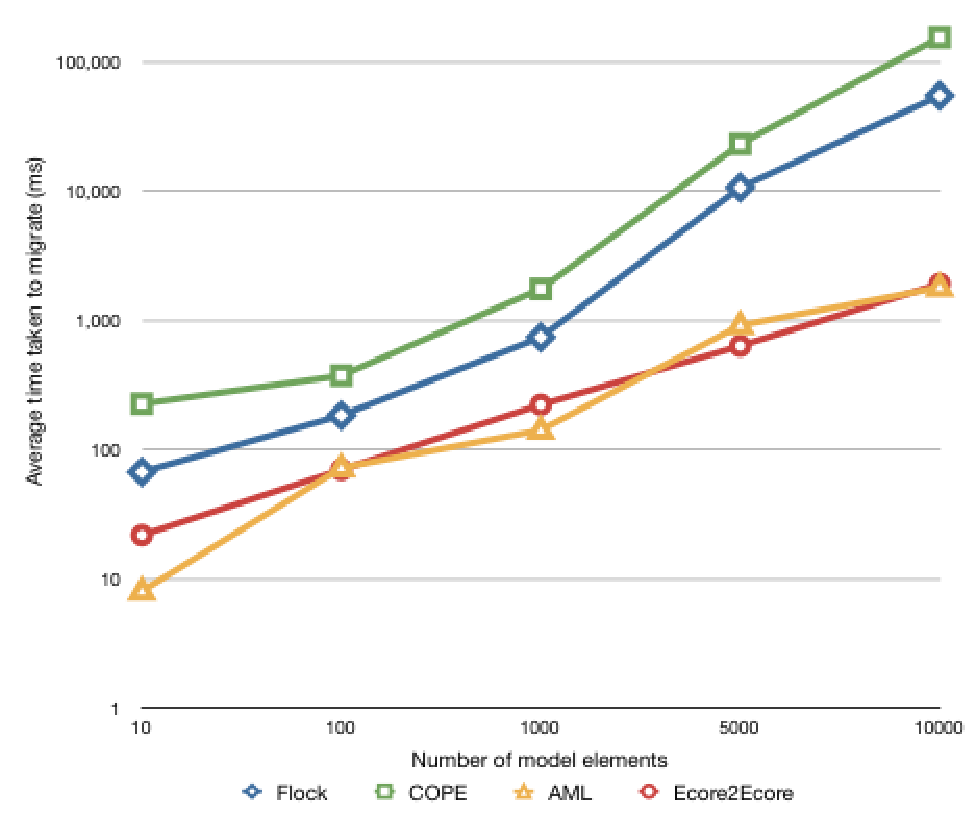
\includegraphics[width=10cm]{6.Evaluation/images/migration_tool_performance.pdf}
	\caption{Migration tool performance comparison.}
	\label{fig:performance}
\end{figure}

To measure performance, five sets of Petri net models were generated at random. Models in each set contained 10, 100, 1000, 5,000, and 10,000 model elements.  Figure~\ref{fig:performance} shows the average time taken by each tool to execute migration across 10 repetitions for models of different sizes. Note that the Y axis has a logarithmic scale. The results indicate that, for the Petri nets co-evolution example, AML and Ecore2Ecore execute migration significantly more quickly than COPE and Flock, particularly when the model to be migrated contains more than 1,000 model elements. Figure~\ref{fig:performance} indicates that, for the Petri nets co-evolution example, Flock executes migration between two and three times faster than COPE, although the author of COPE reports that turning off validation causes COPE to perform similarly to Flock.


\subsection{Discussion}
\label{sec:discussion}
The comparison described above highlights similarities and differences between a representative sample of model migration approaches. From this comparison, guidance for selecting between tools was synthesised. The guidance is presented below, and was produced by all four participants in the comparison (Herrmannsd\"{o}rfer, Williams, Kolovos and the author). 

COPE captures co-evolution patterns (which apply to both model and metamodel), while Ecore2Ecore, AML and Flock capture only model migration patterns (which apply just to models). Because of this, COPE facilitates a greater degree of re-use in model migration than other approaches. However, the order in which the user applies patterns with COPE impacts on both metamodel evolution and model migration, which can complicate pattern selection particularly when a large amount of evolution occurs at once. The re-usable co-evolution patterns in COPE make it well suited to migration problems in which metamodel evolution is frequent and in small steps.

Flock, AML and Ecore2Ecore are preferable to COPE when metamodel evolution has occurred before the selection of a migration approach. Because of its use of co-evolution patterns, we conclude that COPE is better suited to forward- rather than reverse-engineering.

Through its Convergence View and integration with the EMF metamodel editor, COPE facilitates metamodel analysis that is not possible with the other approaches considered in this paper. COPE is well-suited to situations in which measuring and reasoning about co-evolution is important.

In situations where migration involves modelling technologies other than EMF, AML and Flock are preferable to COPE and Ecore2Ecore. AML can be used with models represented in KM3, while Flock can be used with models represented in MDR, XML and CZT. Via the connectivity layer of Epsilon, Flock can be extended to support further modelling technologies.

There are situations in which Ecore2Ecore or AML might be preferable to Flock and COPE. For large models, Ecore2Ecore and AML might execute migration significantly more quickly than Flock and COPE. Ecore2Ecore is the only tool that has no technical dependencies (other than a modelling framework). In situations where migration must be embedded in another tool, Ecore2Ecore offers a smaller footprint than other migration approaches. Compared to the other approaches considered in this paper, AML automatically generates migration strategies with the least guidance from the user.

Despite these advantages, Ecore2Ecore and AML are unsuitable for some types of migration problem, because they are less expressive than Flock and COPE. Specifically, changes to the containment of model elements typically cannot be expressed with Ecore2Ecore and changes that are classified by %\cite{gruschko07towards} as \emph{breaking and non-resolvable}
\cite{herrmannsdoerfer08automatability} as \emph{metamodel-specific}
cannot be expressed with AML. Because of this, it is important to investigate metamodel changes before selecting a migration tool. Furthermore, it might be necessary to anticipate which types of metamodel change are likely to arise before selecting a migration tool. Investing in one tool to discover later that it is no longer suitable causes wasted effort.

\begin{table}[hbtp]
	\centering
	\begin{tabular}{|c|c|}
	\hline
	\textbf{Requirement}    & \textbf{Recommended Tools} \\
	\hline
	Frequent, incremental co-evolution                & COPE \\
	\hline
	Reverse-engineering                               & AML, Ecore2Ecore, Flock \\
	\hline
	Modelling technology diversity                    & Flock \\
	\hline
	Quicker migration for larger models               & AML, Ecore2 Ecore \\
	\hline
	Minimal dependencies                              & Ecore2Ecore \\
	\hline
	Minimal hand-written code                         & AML, COPE \\
	\hline
	Minimal guidance from user                        & AML \\
	\hline
	Support for metamodel-specific migrations   & COPE, Flock \\
%	Support for breaking and non-resolvable changes   & COPE, Flock \\
	\hline
	\end{tabular}
	\caption[Summary of tool selection advice]{Summary of tool selection advice. (Tools are ordered alphabetically).}
	\label{tab:advice}
\end{table}

\subsubsection{Strengths and Weaknesses of Flock}
The comparison and guidance highlight strengths and weaknesses of AML, COPE, Ecore2Ecore and Flock. The findings for Flock are now summarised.

\paragraph{Strengths} Flock was the only co-evolution tool suitable for performing model migration when the original and evolved metamodels are specified in different modelling technologies. AML, Ecore2Ecore and COPE are interoperable with a single modelling technology, the Eclipse Modelling Framework. Migrating models between metamodels represented in different modelling technologies would require modification of the co-evolution tool when using AML, Ecore2Ecore or COPE and hence, model migration with Flock requires less effort than using AML, Ecore2Ecore or COPE when migrating between modelling technologies. This was a key requirement for the co-evolution example described in the sequel.

For the examples of metamodel evolution explored here, Flock (and COPE) is more expressive than AML, but requires more guidance from the user. This is consistent with the trade-off between flexibility and level of automation of co-evolution approaches identified in Chapter~\ref{Analysis}.

Unlike COPE, Flock (and AML and Ecore2Ecore) does not make assumptions on the way in which metamodel evolution will be specified. With Flock, AML and Ecore2Ecore, metamodel evolution need not occur at the same time or in the same development environment as the formulation of the model migration strategy. For this reason, Flock (and AML and Ecore2Ecore) arguably lead to more productive model migration when used to formulate a model migration strategy after metamodel evolution has already been specified, as was the case for the GMF Graph example used in this section.

\paragraph{Weaknesses} The results presented here indicate that model migration with Flock takes longer to execute than with AML and Ecore2Ecore. This is likely because Flock migration strategies are interpreted, while AML and Ecore2Ecore migration strategies are compiled. A compiler for Flock would likely increase execution time, but, at present, Epsilon, the platform atop which Flock is built, lacks the infrastructure required for constructing compilers. As such, model migration with Flock is likely to be less productive than with AML or Ecore2Ecore when a large models or a large number of models are to be migrated.

Compared to COPE and AML, Flock lacks re-use of model migration patterns across varying metamodels. In Flock, model migration is specified in terms of concrete metamodel types and cannot be re-used for different metamodels. By contrast, COPE and AML capture model migration in a metamodel-independent manner. When migration is likely to be a commonly occurring practice, the use of COPE or AML rather than Flock is likely to led to increased productivity of model migration, because the metamodel-independent migration patterns will likely increase re-use and provide a vocabulary for describing migration. Section~\ref{sec:future_work} describes ways in which Flock might be extended to capture metamodel-independent migration patterns.

\subsection{Summary}
The work presented in this section compared a representative sample of approaches to automating developer-driven co-evolution using an expert evaluation. The comparison was performed by following a methodical process and using an example from a real-world MDE project. Some preliminary recommendations and guidelines in choosing a co-evolution tool were synthesised from the presented results and are summarised in Table~\ref{tab:advice}. The comparison was carried out by the tool developers (or stand-ins where the developers were unable to participate fully). Each developer used a tool other than their own so that the comparison could more closely emulate the level of expertise of a typical user.

The results of the comparison suggested situations in which the use of Flock might lead to increased productivity of model migration, and, conversely, situations in which an alternative tool might be preferable. The comparison results suggest that Flock is well-suited to co-evolution when models are to be migrated between different modelling technologies, when migration involves metamodel-specific detail, and when metamodel evolution has occurred prior to -- or in a different development environment to -- the formulation of a model migration strategy. Additionally, Flock might be improved via optimisations to increase the execution time of large models or a large number of models, and by considering the ways in which model migration patterns could be captured in a metamodel-independent manner.

Some criteria were excluded from the comparison because of the method employed. For instance, the learnability of a tool affects the productivity of users, and, as such, affects tool selection. However, drawing conclusions about learnability (and also productivity and usability) is challenging with the comparison method employed because of the subjective nature of these characteristics. A comprehensive user study (with hundreds of users) would be more suitable for assessing these types of criteria.

%!TEX root = /Users/louis/Documents/PhD/Deliverables/Thesis/thesis.tex
\section[Evaluating Co-Evolution Tools with an Example from UML][Evaluating Co-Evolution Tools (UML)]{Evaluating Co-Evolution Tools with an Example from UML}
\label{sec:ttc}
In contrast to the previous section, which compared Flock to three co-evolution tools, the evaluation performed in this section compares Flock with model-to-model transformation tools. As discussed in Chapter~\ref{Analysis}, model migration can be regarded as a specialisation of model-to-model transformation. Chapter~\ref{Implementation} introduces Flock, a language tailored for model migration. This section compares Flock with other model-to-model transformation languages, and explores the benefits and drawbacks of treating model migration and model-to-model transformation as separate model management operations, as proposed in this thesis and by \cite{sprinkle03thesis}.

The author participated in the 2010 edition of the Transformation Tools Contest (TTC), a workshop series that seeks to compare and contrast tools for performing model and graph transformation. At TTC 2010\footnote{\url{http://www.planet-research20.org/ttc2010/index.php?Itemid=132}}, two rounds of submissions were invited: cases (transformation problems, three of which are selected by the workshop organisers) and solutions to the selected cases. The author submitted a case based on a model migration problem from a real-world example of metamodel evolution. Nine solutions were submitted for the case, including one by the author, which used Flock.

Compared to the evaluation described in Section~\ref{sec:collaborative_comparison}, the evaluation in this section compares Flock to a wider range of tools (model and graph transformation tools, and not just model migration tools). The remainder of this section describes the model migration case (Section~\ref{subsec:ttc_case}), the Flock solution (Section~\ref{subsec:ttc_solution}), and reports the results of the workshop in which the solutions were compared and scored by the organisers and participants.


\subsection{Model Migration Case}
\label{subsec:ttc_case}
To compare Flock with other transformation tools for specifying model migration, the author submitted a case to TTC based on the evolution of the UML. The way in which activity diagrams are modelled in the UML changed significantly between versions 1.4 and 2.1 of the specification. In the former, activities were defined as a special case of state machines, while in the latter they are defined with a more general semantic base\footnote{A variant of generalised coloured Petri nets.} \cite{selic05uml2}.

The remainder of this section briefly introduces UML activity diagrams, describes their evolution, and discusses the way in which solutions were assessed. Section~\ref{subsec:uml_activity_diagrams} describes the metamodel evolution in more detail. The work presented in this section is based on the case submitted to TTC 2010 \cite{rose10ttc_case}. 

\subsubsection{Activity Diagrams in UML}
Activity diagrams are used for modelling lower-level behaviours, emphasising sequencing and co-ordination conditions. They are used to model business processes and logic \cite{uml22}. Figure~\ref{fig:activity} shows an activity diagram for filling orders. The diagram is partitioned into three \emph{swimlanes}, representing different organisational units. \emph{Activities} are represented with rounded rectangles and \emph{transitions} with directed arrows. \emph{Fork} and \emph{join} nodes are specified using a solid black rectangle. \emph{Decision} nodes are represented with a diamond. Guards on transitions are specified using square brackets. For example, in Figure~\ref{fig:activity} the transition to the restock activity is guarded by the condition \texttt{[not in stock]}. Text on transitions that is not enclosed in square brackets represents a trigger event. In Figure~\ref{fig:activity}, the transition from the restock activity occurs on receipt of the asynchronous signal called \texttt{receive stock}. Finally, the transitions between activities might involve interaction with objects. In Figure~\ref{fig:activity}, the Fill Order activity leads to an interaction with an object called \texttt{Filled Object}. 

\begin{figure}[htbp]
  \centering
  \includegraphics*[viewport=75 230 585 800,width=13cm]{6.Evaluation/images/activity.pdf}
  \caption[Activity model in UML 1.4.]{Activity model in UML 1.4, taken from \cite{rose10ttc_case} and based on \cite[pg3-165]{uml14}.}
  \label{fig:activity}
\end{figure}

Between versions 1.4 and 2.2 of the UML specification, the metamodel for activity diagrams has changed significantly. The \cc sequel summarises most of the changes, and further details can be found in the UML 1.4 \cite{uml14} and UML 2.2 \cite{uml22} specifications.

\subsubsection{Evolution of Activity Diagrams}
Figures~\ref{fig:uml14} and \ref{fig:uml22} are simplifications of the activity diagram metamodels from versions 1.4 and 2.2 of the UML specification, respectively. In the interest of clarity, some features and abstract classes have been removed from Figures~\ref{fig:uml14} and \ref{fig:uml22}.

Some differences between Figures~\ref{fig:uml14} and \ref{fig:uml22} are: activities have been changed such that they comprise nodes and edges, actions replace states in UML 2.2, and the subtypes of control node replace pseudostates.

\begin{figure}[htbp]
  \centering
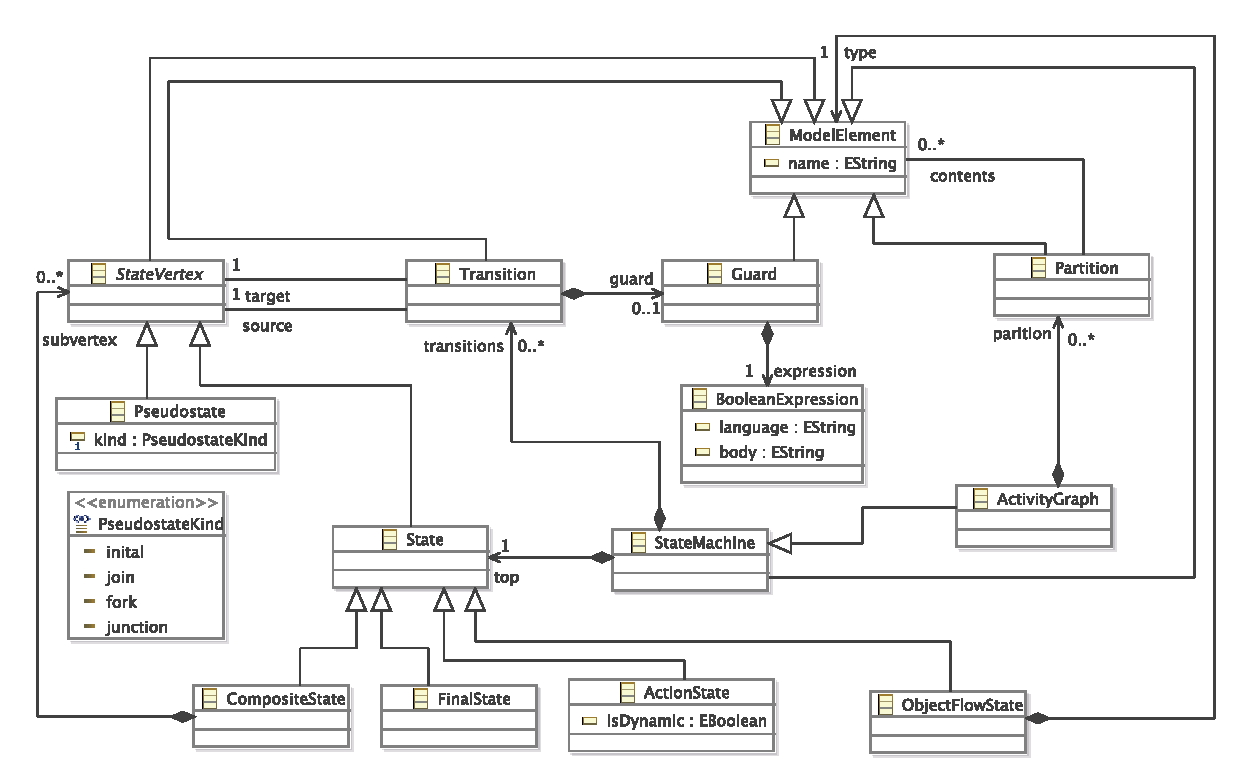
\includegraphics[width=12cm]{A.3.MigrationStrategies/images/uml/activity_diagrams_before.pdf}
  \caption[UML 1.4 Activity Graphs]{UML 1.4 Activity Graphs (based on \cite{uml14}).}
  \label{fig:uml14}
\end{figure} 

\begin{figure}[htbp]
  \centering
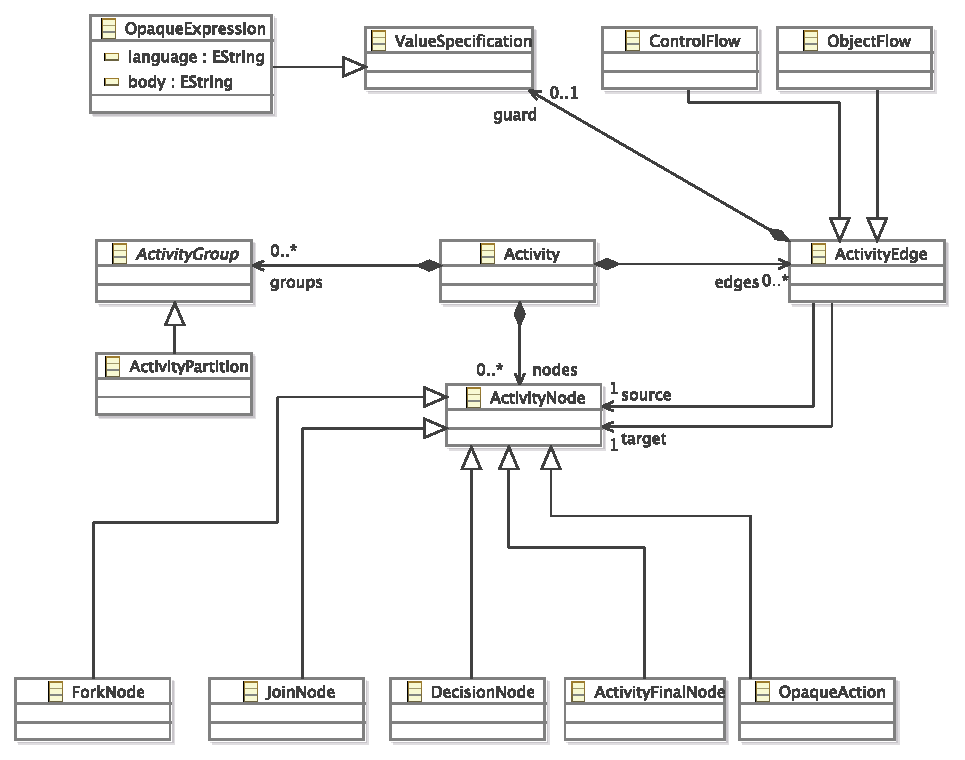
\includegraphics[width=12cm]{A.3.MigrationStrategies/images/uml/activity_diagrams_after.pdf}
  \caption[UML 2.2 Activity Diagrams]{UML 2.2 Activity Diagrams (based on \cite{uml22}).}
  \label{fig:uml22}
\end{figure}

To facilitate the comparison of solutions, the model shown in Figure~\ref{fig:activity} was used. Solutions migrated the activity diagram shown in Figure~\ref{fig:activity} -- which conforms to UML 1.4 -- to conform to UML 2.2. The UML 1.4 model, the migrated UML 2.2 model, and the UML 1.4 and 2.2 metamodels are available from\footnote{\url{http://www.cs.york.ac.uk/~louis/ttc/}}.

Submissions were evaluated using the following criteria, which were decided in advance by the author and the workshop organisers:

\begin{itemize}
	\item \textbf{Correctness}: Does the transformation produce a model equivalent to the migrated UML 2.2. model included in the case resources?
	\item \textbf{Conciseness}: How much code is required to specify the transformation? (Sprinkle \cc and Karsai propose that the amount of effort required to codify migration should be directly proportional to the number of changes between original and evolved metamodel \cite{sprinkle04domain}).
		\item \textbf{Clarity}: How easy is it to read and understand the used transformation? (For example, is a well-known or standardised language?)
		\item \textbf{Appropriateness}: How much effort is required to adapt the tool in providing a solution?
		\item \textbf{Tool maturity}: To what extent can the tool be used by people other than the developer? 
		\item \textbf{Reproducibility}: Can the solution be reproduced on another machine?\footnote{Participants were invited to install their tools and solutions on virtual machines, which would later be made accessible via the workshop proceedings.}
		\item \textbf{Extensions}: Which of the case extensions (described below) were implemented in the solution?
\end{itemize}

To further distinguish between solutions, three extensions to the core task were proposed. The first extension was added after the case was submitted, and was proposed by the workshop organisers and the solution authors. The second and third extension were included in the case by the author. 

\subsubsection{Extension 1: Alternative Object Flow State Migration Semantics}
\label{sub:object_flow_states}
Following the submission of the case to the competition, discussion on the TTC forums\footnote{\url{http://planet-research20.org/ttc2010/index.php?option=com_community&view=groups&task=viewgroup&groupid=4&Itemid=150} (registration required)} revealed an ambiguity in the UML 2.2 specification indicating that the migration semantics for the ObjectFlowState UML 1.4 concept are not clear from the UML 2.2 specification. The case was revised to incorporate both the original semantics (suggested by the author and described above) and an alternative semantics (suggested by a workshop participant via the TTC forums) for migrating \texttt{Ob\-je\-ctFl\-owSt\-a\-t\-es}. The alternative semantics are now described.

\textbf{In the core task} described above, instances of \texttt{Ob\-je\-ctFl\-owSt\-a\-te} were migrated to instances of \texttt{Ob\-je\-ctNo\-de}. Any instances of \texttt{Tr\-an\-si\-ti\-on} that had an \texttt{Ob\-je\-ctFl\-owSt\-a\-te} as their source or target were migrated to instances of \texttt{Ob\-je\-ctFl\-ow}. Figure~\ref{fig:ofs_to_node} shows an example application of this migration semantics. Structures such as the one shown in Figure~\ref{fig:ofs_to_node_before} are migrated to an equivalent structure shown in Figure~\ref{fig:ofs_to_node_after}. The \texttt{Tr\-an\-si\-ti\-on}s, \texttt{t1} and \texttt{t2}, are migrated to instances of \texttt{Ob\-je\-ctFl\-ow}. Likewise, the instance of \texttt{Ob\-je\-ctFl\-owSt\-a\-te}, \texttt{s2}, is migrated to an instance of \texttt{Ob\-je\-ctNo\-de}.

\begin{figure}[htbp]
	\centering
	\subfigure[ObjectFlowState structure in UML 1.4]
	{
	    \label{fig:ofs_to_node_before}
	    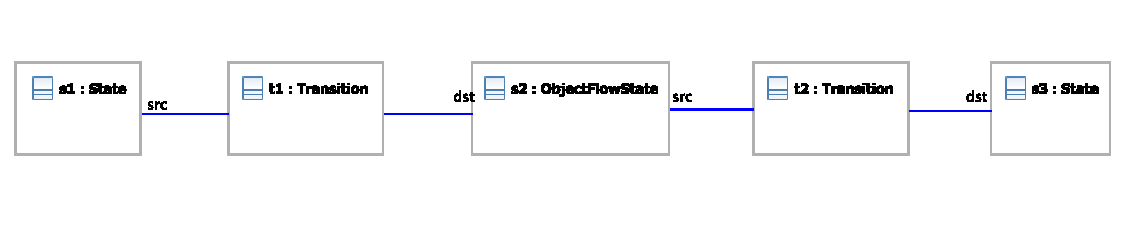
\includegraphics[height=2.5cm]{6.Evaluation/images/ttc/core_before.pdf}
	}
	\subfigure[Equivalent ObjectNode structure in UML 2.2]
	{
	    \label{fig:ofs_to_node_after}
	    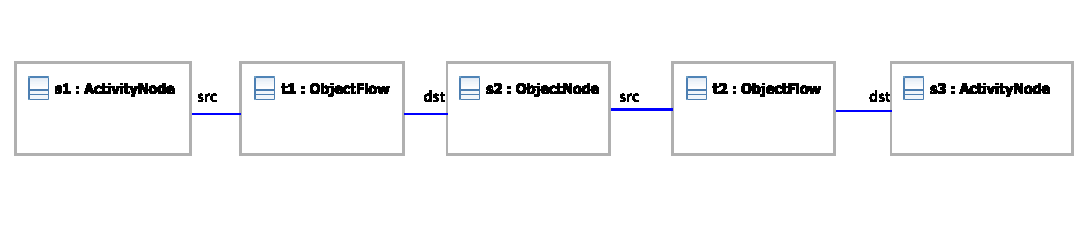
\includegraphics[height=2.5cm]{6.Evaluation/images/ttc/core_after.pdf}
	}
	\caption{Migrating Actions for the Core Task}
\label{fig:ofs_to_node}
\end{figure}


\textbf{This extension} considered an alternative migration semantics for ObjectFlowState. For this extension, instances of \texttt{Ob\-je\-ctFl\-owSt\-a\-te} (and any connected \texttt{Tr\-an\-si\-ti\-on}s) were migrated to instances of  \texttt{Ob\-je\-ctFl\-ow}, as shown in Figure~\ref{fig:ofs_to_flow} in which the UML 2.2 \texttt{Ob\-je\-ctFl\-ow}, \texttt{f1}, replaces \texttt{t1}, \texttt{t2} and \texttt{s2}.

\begin{figure}[htbp]
	\centering
	\subfigure[ObjectFlowState structure in UML 1.4]
	{
	    \label{fig:ofs_to_flow_before}
	    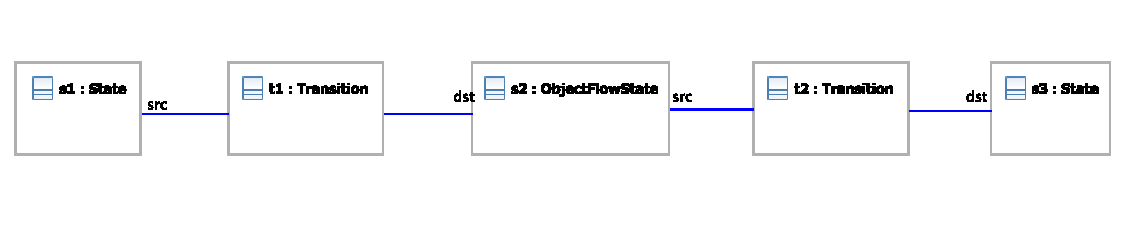
\includegraphics[height=2.5cm]{6.Evaluation/images/ttc/core_before.pdf}
	}
	\subfigure[Equivalent ObjectFlow structure in UML 2.2]
	{
	    \label{fig:ofs_to_flow_after}
	    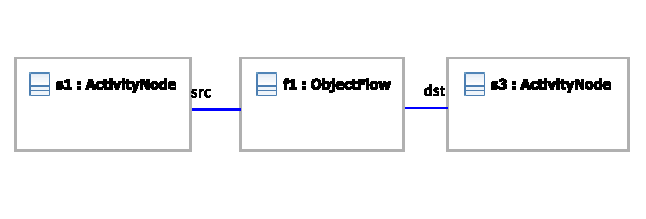
\includegraphics[height=2.5cm]{6.Evaluation/images/ttc/ext_after.pdf}
	}
	\caption{Migrating Actions for Extension 1}
\label{fig:ofs_to_flow}
\end{figure}

\subsubsection{Extension 2: Concrete Syntax}
\label{sub:concrete_syntax}
The second extension relates to the appearance of activity diagrams. The UML specifications provide no formally defined metamodel for the concrete syntax of UML diagrams. However, some UML tools store diagrammatic information in a structured manner using XML or a modelling tool. For example, the Eclipse UML 2 tools\footnote{\url{http://www.eclipse.org/modeling/mdt/?project=uml2tools}} store diagrams as GMF \cite{gronback09emp} diagram models.

Submissions were invited to explore the feasibility of migrating the concrete syntax of the activity diagram shown in Figure~\ref{fig:activity} to the concrete syntax in their chosen UML 2 tool. To facilitate this, the case resources included an ArgoUML project\footnote{\url{http://argouml.tigris.org/}} containing the activity diagram shown in Figure~\ref{fig:activity}.

\subsubsection{Extension 3: XMI}
\label{sub:xmi}
The UML specifications \cite{uml14,uml22} indicate that UML models should be stored using XMI. However, because XMI has evolved at the same time as UML, UML 1.4 tools most likely produce XMI of a different version to UML 2.2 tools. For instance, ArgoUML produces XMI 1.2 for UML 1.4 models, while the Eclipse UML2 tools produce XMI 2.1 for UML 2.2.

As an extension to the core task, submissions were invited to consider how to migrate a UML 1.4 model represented in XMI 1.x to a UML 2.1 model represented in XMI 2.x. To facilitate this, the UML 1.4 model shown in Figure~\ref{fig:activity} was made available in XMI 1.2 as part of the case resources.

Following the submission of the case, Tom Morris, the project leader for ArgoEclipse and a committer on ArgoUML, encouraged solutions to consider the extension described above. ArgoUML cannot, at present, migrate models from UML 1 to UML 2.  On the TTC forums, Morris stated that ``We have nothing available to fill this hole currently, so any contributions would be hugely valuable.  Not only would achieve academic fame and glory from the contest, but you'd get to see your code benefit users of one of the oldest (10+ yrs) open source UML modeling tools.'' \footnote{\url{http://www.planet-research20.org/ttc2010/index.php?option=com_community&view=groups&task=viewdiscussion&groupid=4&topicid=20&Itemid=150} (registration required)}

\subsection{Model Migration Solution in Epsilon Flock}
\label{subsec:ttc_solution}
This section describes a Flock solution for migrating UML activity diagrams in response to the evolution described above. The solution was developed by the author, and, at the workshop, compared with migration strategies written in other languages. The workshop participants and organisers rated each tool.

The Flock migration strategy was developed in an iterative and incremental manner, using the following process, starting with an empty migration strategy:

\begin{enumerate}
	\item Execute Flock on the original model, producing a migrated model.
	\item Compare the migrated model with the reference model provided in the case resources.
	\item Change the Flock migration strategy.
	\item Repeat until the migrated and reference models were the same.
\end{enumerate}

The remainder of this section presents the Flock solution in an incremental manner. The code listings in this section show only those rules relevant to the iteration being discussed.

\subsubsection{Actions, Transitions and Final States}
Development of the migration strategy began by executing an empty Flock migration strategy on the original model. Because Flock automatically copies model elements that have not been affected by evolution, the resulting model contained \texttt{Ps\-eu\-do\-st\-at\-e}s and \texttt{Tr\-an\-si\-ti\-on}s, but none of the \texttt{Ac\-ti\-onSt\-a\-te}s from the original model. In UML 2.2 activities, \texttt{Op\-aq\-ueAc\-ti\-on}s replace \texttt{Ac\-ti\-onSt\-a\-te}s. Listing~\ref{lst:actions} shows the Flock code for changing \texttt{Ac\-ti\-onSt\-a\-te}s to corresponding \texttt{Op\-aq\-ueAc\-ti\-on}s.

\begin{lstlisting}[caption=Migrating Actions, label=lst:actions, language=Flock]
migrate ActionState to OpaqueAction
\end{lstlisting}

Next, similar rules were added to migrate instances of \texttt{FinalState} to instances of \texttt{ActivityFinalNode} and to migrate instances of \texttt{Transition} to \texttt{ControlFlow}, as shown in Listing~\ref{lst:final_states}.

\begin{lstlisting}[caption=Migrating FinalStates and Transitions, label=lst:final_states, language=Flock]
migrate FinalState to ActivityFinalNode
migrate Transition to ControlFlow
\end{lstlisting}

\subsubsection{Pseudostates}
Development continued by selecting further types of state that were not present in the migrated model, such as \texttt{Ps\-eu\-do\-st\-at\-es}s, which are not used in UML 2.2 activities. Instead, UML 2.2 activities use specialised \texttt{No\-de}s, such as \texttt{In\-it\-ialNo\-de}. Listing~\ref{lst:pseudostates} shows the Flock code used to change \texttt{Ps\-eu\-do\-st\-a\-te}s to corresponding \texttt{No\-de}s.

\begin{lstlisting}[caption=Migrating Pseudostates, label=lst:pseudostates, language=Flock]
migrate Pseudostate to InitialNode  when: original.kind = Original!PseudostateKind#initial
migrate Pseudostate to DecisionNode when: original.kind = Original!PseudostateKind#junction
migrate Pseudostate to ForkNode     when: original.kind = Original!PseudostateKind#fork
migrate Pseudostate to JoinNode     when: original.kind = Original!PseudostateKind#join
\end{lstlisting}

\subsubsection{Activities}
In UML 2.2, \texttt{Ac\-ti\-vi\-ty}s no longer inherit from state machines. As such, some of the features defined by \texttt{Ac\-ti\-vi\-ty} have been renamed. Specifically, \texttt{tr\-an\-si\-ti\-o\-ns} has become \texttt{ed\-g\-es} and \texttt{par\-ti\-ti\-o\-ns} has become \texttt{gr\-o\-u\-ps}. Furthermore, the states (or nodes in UML 2.2 parlance) of an \texttt{Ac\-ti\-vi\-ty} are now contained in a feature called \texttt{nodes}, rather than in the \texttt{su\-bv\-er\-t\-ex} feature of a composite state accessed via the \texttt{top} feature of \texttt{Ac\-ti\-vi\-ty}. The Flock migration rule shown in Listing~\ref{lst:activities} captured these changes.

\begin{lstlisting}[caption=Migrating ActivityGraphs, label=lst:activities, language=Flock]
migrate ActivityGraph to Activity {
	migrated.edge  = original.transitions.equivalent();
	migrated.group = original.partition.equivalent();
	migrated.node  = original.top.subvertex.equivalent();
}
\end{lstlisting}

Note that the rule in Listing~\ref{lst:activities} used the built-in \texttt{eq\-ui\-va\-le\-nt} operation to find migrated model elements from original model elements. As discussed in Section~\ref{sec:flock}, the \texttt{equ\-iv\-al\-e\-nt} operation invokes other migration rules where necessary and caches results to improve performance.

Next, a similar rule for migrating \texttt{Gu\-ar\-d}s was added. In UML 1.4, the the \texttt{gu\-a\-rd} feature of \texttt{Tr\-an\-si\-ti\-on} references a \texttt{Gu\-a\-rd}, which in turn references an \texttt{Ex\-pr\-es\-si\-on} via its \texttt{ex\-pr\-es\-si\-on} feature. In UML 2.2, the \texttt{gu\-a\-rd} feature of \texttt{Tr\-an\-si\-ti\-on} references an \texttt{Op\-aq\-ueEx\-pr\-es\-si\-on} directly. Listing~\ref{lst:guards} captures this in Flock.

\begin{lstlisting}[caption=Migrating Guards, label=lst:guards, language=Flock]
migrate Guard to OpaqueExpression {
	migrated.body.add(original.expression.body);
}

\end{lstlisting}


\subsubsection{Partitions}
In UML 1.4 activity diagrams, \texttt{Pa\-rt\-it\-i\-on} specifies a single containment reference for its \texttt{co\-nt\-en\-ts}. In UML 2.2 activity diagrams, partitions have been renamed to \texttt{ActivityPartition}s and specify two containment features for their contents, \texttt{ed\-g\-es} and \texttt{no\-d\-es}. Listing~\ref{lst:partitions} shows the rule used to migrate \texttt{Pa\-rt\-it\-i\-on}s to \texttt{Ac\-ti\-vi\-tyPa\-rt\-it\-i\-on}s in Flock. The body of the rule shown in Listing~\ref{lst:partitions} uses the \emph{collect} operation to segregate the \texttt{co\-nt\-en\-ts} feature of the original model element into two parts.

\begin{lstlisting}[caption=Migrating Partitions, label=lst:partitions, language=Flock]
migrate Partition to ActivityPartition {
	migrated.edges = original.contents.collect(e:Transition | e.equivalent());
	migrated.nodes = original.contents.collect(n:StateVertex | n.equivalent());	
}
\end{lstlisting}


\subsubsection{ObjectFlows}
Finally, two rules were written for migrating model elements relating to object flows. In UML 1.4 activity diagrams, object flows are specified using \texttt{Ob\-je\-ctFl\-owSt\-a\-te}, a subtype of \texttt{St\-at\-eVe\-rt\-ex}. In UML 2.2 activity diagrams, object flows are modelled using a subtype of \texttt{ObjectNode}. In UML 2.2 flows that connect to and from \texttt{Ob\-je\-ctNo\-de}s must be represented with \texttt{Ob\-je\-ctFl\-ow}s rather than \texttt{Co\-nt\-rolFl\-ow}s.

Listing~\ref{lst:objectflows} shows the Flock rule used to migrate \texttt{Tr\-an\-si\-ti\-on}s to \texttt{Ob\-je\-ctFl\-ow}s. The rule applies for \texttt{Tr\-an\-si\-ti\-on}s whose source or target \texttt{St\-at\-eVe\-rt\-ex} is of type \texttt{Ob\-je\-ctFl\-owSt\-ate}.

\begin{lstlisting}[caption=Migrating ObjectFlows, label=lst:objectflows, language=Flock]
migrate ObjectFlowState to ActivityParameterNode

migrate Transition to ObjectFlow when: original.source.isTypeOf(ObjectFlowState) or original.target.isTypeOf(ObjectFlowState)
\end{lstlisting}

In addition to the core task, the Flock solution also approached two of the three extensions described in the case (Section~\ref{subsec:ttc_case}). The solutions to the extensions are now discussed.

\subsubsection{Alternative ObjectFlowState Migration Semantics}
The first extension required submissions to consider an alternative migration semantics for \texttt{Ob\-je\-ctFl\-owSt\-a\-te}, in which a single \texttt{Ob\-je\-ctFl\-ow} replaces each \texttt{Ob\-je\-ctFl\-owSt\-a\-te} and any connected \texttt{Tr\-an\-si\-ti\-on}s.

Listing~\ref{lst:objectflows2} shows the Flock source code used to migrate \texttt{Ob\-je\-ctFl\-owSt\-at\-es} (and connecting \texttt{Tr\-an\-si\-ti\-on}s) to a single \texttt{Ob\-je\-ctFl\-ow}. This rule was used instead of the two rules defined in Listing~\ref{lst:objectflows}. In the body of the rule shown in Listing~\ref{lst:objectflows2}, the \texttt{so\-ur\-ce} of the \texttt{Tr\-an\-si\-ti\-on} is copied directly to the \texttt{so\-u\-rce} of the \texttt{Ob\-je\-ctFl\-ow}. The \texttt{ta\-rg\-et} of the \texttt{Ob\-je\-ctFl\-ow} is set to the target of the first outgoing \texttt{Tr\-an\-si\-ti\-on} from the \texttt{Ob\-je\-ctFl\-owSt\-a\-te}. 

\begin{lstlisting}[caption=Migrating ObjectFlowStates to a single ObjectFlow, label=lst:objectflows2, language=Flock]
migrate Transition to ObjectFlow when: original.target.isTypeOf(ObjectFlowState) {
	migrated.source = original.source.equivalent();
	migrated.target = original.target.outgoing.first.target.equivalent();
}
\end{lstlisting}

Because, in this alternative semantics, \texttt{Ob\-je\-ctFl\-owSt\-a\-te}s are represented as edges rather than nodes, the partition migration rule was changed such that \texttt{Ob\-je\-ctFl\-owSt\-a\-te}s were not copied to the \texttt{no\-des} feature of \texttt{Pa\-rt\-it\-i\-on}s. To filter out the \texttt{Ob\-je\-ctFl\-owSt\-a\-te}s, line 3 of Listing~\ref{lst:partitions} was changed to include a reject statement, as shown on line 3 of Listing~\ref{lst:partitions2}.

\begin{lstlisting}[caption=Migrating Partitions without ObjectFlowStates, label=lst:partitions2, language=Flock]
migrate Partition to ActivityPartition {
	migrated.edges = original.contents.collect(e:Transition | e.equivalent());
	migrated.nodes = original.contents.reject(ofs:ObjectFlowState | true).collect(n:Original!StateVertex | n.equivalent());	
}
\end{lstlisting}

The complete source code listing for the Flock migration strategy is provided in Section~\ref{subsec:uml_activity_diagrams}.

\subsubsection{XMI}
\label{sec:xmi}
The second extension required submissions to migrate an activity graph conforming to UML 1.4 and encoded in XMI 1.2 to an equivalent activity graph conforming to UML 2.2 and encoded in XMI 2.1. The core task did not require submissions to consider changes to XMI (the model storage representation), but, in practice, this is a challenge to migration, as noted by Tom Morris on the TTC forums\footnote{\url{http://www.planet-research20.org/ttc2010/index.php?option=com_community&view=groups&task=viewdiscussion&groupid=4&topicid=20&Itemid=150} (registration required)}.

As discussed in Section~\ref{sec:flock}, Flock extends and reuses \changed{``is built atop'' changed to ``extends and reuses''} Epsilon, which includes a model connectivity layer (EMC). EMC provides a common interface for accessing and persisting models. Currently, EMC supports EMF (XMI 2.x), MDR (XMI 1.x), and plain XML models. To support migration between metamodels defined in heterogeneous modelling frameworks, EMC was extended during the development of Flock to provide a conformance checking service.

Consequently, the migration strategy developed for the core task works for all of the types of model supported by EMC. To migrate a model encoded in XMI 1.2 rather than in XMI 2.1, the user must select a different option when executing the Flock migration strategy. Otherwise, no other changes are required.

\subsection{Comparison with other solutions}
At the workshop, solutions to the migration case described in Section~\ref{subsec:ttc_case} were presented. Each solution was allocated two opponents who highlighted weaknesses of each approach. Following the solution presentations and opposition statements, each solution was scored using the criteria described above: correctness, clarity, conciseness, appropriateness, tool maturity, reproducibility and number of extensions solved. Flock scored the highest average marks for four of seven criteria, and was awarded overall first prize. The remainder of this section discusses the scores in more detail, and summarises the opposition statements for Flock.

\subsubsection{Opposition Statements}
The opposition statements highlighted two weaknesses of Flock. Firstly, there is some duplicated code in Listing~\ref{lst:pseudostates}: the \texttt{migrate Pseudostate to ...} statement appears several times. The duplication exists because Flock only allows one-to-one mappings between original and evolved metamodel types. The conservative copy algorithm would need to be extended to allow one-to-many mappings to remove this kind of duplication.

Secondly, the body of Flock rules are specified in an imperative manner. Consequently, reasoning about the correctness of a migration strategy is arguably more difficult than in languages that use a purely declarative syntax. This point is discussed further in Section~\ref{sec:limitations}, which considers the limitations of the thesis.

\subsubsection{Scoring}
Flock was awarded the overall first prize and scored the highest average marks for five of the seven criteria outlined above. The overall ranking process is first described, and the remainder of the section discusses the score awarded to Flock for each of the criteria.

During the workshop, each tool developer presented their solution. The workshop participants and organisers awarded each solution an individual score for each of the seven criteria outlined above, and a total score (by summing the seven criteria scores). The overall ranking for each solution was calculated by taking the mean of the total scores. For example, Flock was awarded the scores shown in Table~\ref{tab:flock_scores}. (Note that Participants \#2 and \#3 did not award scores to Flock due to a conflict of interest). Appendix~\ref{TTCScores} presents the complete set of results.

Although Flock was awarded the overall first prize, few conclusions can be drawn from the rankings. The scores for each criterion were awarded on different scales (e.g. -2 to 2 for conciseness, and 0 to 2 for extensions) and the workshop organisers applied a weight to each criterion before calculating the totals (5 for correctness; 4 for tool maturity; 3 for conciseness, clarity, extensions, and appropriateness; and 2 for reproducibility). Clearly, the relative importance of each criterion may vary between migration cases, and between organisations. Therefore, the remainder of the discussion focusses on the per-criteria scores awarded to Flock and the other tools.

\begin{table}[tbp]
	\centering
	\begin{tabular}{|r|c|c|c|c|c|c|c|c|c|c|c|}
		\hline
		\textbf{Response \#} & \textbf{1} & \textbf{4} & \textbf{5} & \textbf{6} & \textbf{7} & \textbf{8} & \textbf{9} & \textbf{10} & \textbf{11} & \textbf{12} & \textbf{Mean} \\
		\hline
		\hline
		Correctness          & 0          & 1          & 1          & 1          & 0          & 0          & 1          & 1     
		        & 1           & 1           & \\
		\hline                                                                                                     
		Conciseness          & 1          & 2          & 2          & 1          & 1          & 1          & 0          & 1
		        & 2           & 1           & \\
		\hline                                                                                                     
		Clarity              & 1          & 1          & 1          & 0          & 1          & 1          & 1          & 1
		        & 1           & 1           & \\
		\hline                                                                                                     
		Extensions           & 2          & 2          & 2          & 1          & 2          & 2          & 2          & 2
		        & 2           & 1           & \\
		\hline                                                                                                     
		Appropriateness      & 1         & 2          & 2          & 1          & 2          & 1           & 1          & 2 
		        & 2           & 2           & \\
		\hline                                                                                                     
		Tool Maturity        & 0         & 0          & 0          & 1          & 0          & 0           & 1          & 1
		        & 0           & 1           & \\
		\hline                                                                                                     
		Reproducibility      & 1         & 1          & 1          & 1          & 1          & 1          & 1          & 1 
		        & 1           & 1           & \\
		\hline                                                                                                     
		\hline                                                                                                     
		Total                & 6         & 9          & 9          & 6          & 7          & 6          & 7          & 9 
		        & 9           & 8           & 7.6 \\
		\hline
	\end{tabular}
	\caption{TTC scores for Epsilon Flock (unweighted).}
	\label{tab:flock_scores}
\end{table}

\paragraph{Correctness} Each tool developer demonstrated the extent to which their solution performed a correct migration of activity diagrams according to the migration semantics described in the case description (Section~\ref{subsec:ttc_case}). The following scores could be awarded: -1 (probably doesn't work at all), 0 (cannot judge), 1 (works for one model), and 2 (works for more than one model). Flock received a mean score of 0.7, and was ranked seventh out of the nine solutions. Migration with Flock is specified with both imperative and declarative language constructs, while many of the other solutions use only declarative language constructs to specify the migration of UML activity diagrams and, hence, more could be said about the correctness of the solutions written in those languages.

\paragraph{Conciseness} Solutions were awarded one of the following scores for the conciseness of their migration strategies: -2 (very verbose), -1 (quite verbose), 0 (cannot judges), 1 (quite concise), and 2 (very concise). Flock received a mean score of 1.2, and was ranked first out of the nine solutions. Three of the solutions used general purpose languages (such as Java and Prolog), and these were ranked sixth, seventh and ninth. The other solutions used graph or model transformation languages, and, in general, scored more highly than those written in general-purpose languages.

\paragraph{Clarity} The extent to which the intention of the migration could be determined from the migration strategy was scored on the following scale: -1 (no idea how it works), 0 (some idea how it works), 1 (fully understand how it works). Flock received a mean score of 0.9, was ranked first out of the nine solutions, and there was little variation in the scores awarded to Flock (a score of 1 from eleven of the twelve responses, and a score of 0 from the remaining respondent). Tools tailored to model migration, such as Flock and COPE \cite{herrmannsdoerfer09cope}, and graph transformation languages, such as GrGen \cite{grgen} and MOLA \cite{mola}, were ranked the highest in this category.

\paragraph{Appropriateness} The suitability of the tool for migrating activity diagrams was assessed on the following scale: -2 (totally inappropriate), -1 (inappropriate), 0 (neutral), 1 (somewhat appropriate), 2 (perfect fit). Flock received a mean score of 1.6, and was ranked first out of the nine solutions. Again, tools tailored to model migration, such as Flock and COPE \cite{herrmannsdoerfer09cope}, and graph transformation languages, such as GrGen \cite{grgen} and MOLA \cite{mola}, were ranked the highest in this category.

\paragraph{Tool maturity} The maturity of each tool was discussed during the solution presentations, and the workshop participants were able to use eight of the nine solutions via a virtual machine. Scores were awarded on the following scale: -1 (prototype), 0 (average), 1 (good). Flock received a mean score of 0.4, and was ranked third out of the nine solutions. Fujaba \cite{fujaba} and GrGen \cite{grgen} were ranked first and second in this category, and are established transformation tools that were first reported in the literature in 2000 and 2007 respectively.

\paragraph{Reproducibility} Each developer was invited to configure a virtual machine with their tool and solution, and the workshop participants were invited to use each of the tools. A score of 1 was awarded if a working virtual machine image was provided by the tool developer, and 0 otherwise. Flock had a mean score of 1, and ranked joint first along with seven of the other tools. The virtual machine image for one of the tools did not work, and it was awarded a mean score of 0.

\paragraph{Extensions} Three extensions to the core task were described in Section~\ref{subsec:ttc_case}, and a point was awarded for approaching each additional task. Flock was awarded a mean score of 5.4, and ranked first of the nine solutions. Determining the extensions approached by a solution seems to be an objective task, but some tools were awarded different scores for the extensions criterion which is difficult to explain. For instance, the Flock solution (Section~\ref{subsec:ttc_solution}) approached two of the three extensions, but some of the participants awarded Flock only 1 point. Rather than analysing the scores, it is perhaps more interesting to note that the Flock solution was the only solution to approach the XMI extension, and similarly for Fujaba \cite{fujaba} and the concrete syntax extension. This might indicate that contemporary migration tools can be used to manage realistic metamodel changes, but lack some features that would be desirable in an industrial setting (namely, interoperability with several modelling technologies and co-migration of abstract and concrete syntax).

\subsection{Summary}
This section has discussed the way in which Flock was evaluated by participating in the 2010 edition of the Transformation Tools Contest (TTC). Flock was assessed by application to an example of migration from the UML and comparison with eight other model and graph transformation tools. Flock was awarded the overall first prize and ranked first in five of seven categories by the workshop participants and organisers. 

In addition to evaluating Flock, the work described in this section provides three further contributions. Firstly, the migration case submitted to TTC 2010, described in Section~\ref{subsec:ttc_case} provides a real-world example of co-evolution for use in future comparisons of model migration tools. The case is based on the evolution of UML, between versions 1.4 and 2.2. The migration strategy was devised by analysis of the UML specification, and by discussion between workshop participants.


Secondly, the Flock solution to the migration case (Section~\ref{subsec:ttc_solution}) demonstrates the way in which a migration strategy can be constructed using Flock. In particular, Section~\ref{subsec:ttc_solution} describes an iterative and incremental development process and indicates that an empty Flock migration strategy can provide a useful starting point for development.

Finally, Section~\ref{sec:flock} claims that Flock supports several modelling technologies. The solution described in Section~\ref{subsec:ttc_solution} demonstrates the way in which Flock can be used to migrate models over two modelling technologies: MDR (XMI 1.x) and EMF (XMI 2.x), and hence supports the claim made in Section~\ref{sec:flock}.
%!TEX root = /Users/louis/Documents/PhD/Deliverables/Thesis/thesis.tex

\section{Limitations of the Proposed Structures and Processes}
\label{sec:limitations}
The limitations of the research presented in the thesis are now discussed. Some of the shortcomings identified here are elaborated on in Section~\ref{sec:future_work}, which highlights areas of future work.

\paragraph{Generality} The thesis research focuses on model-metamodel co-evolution, but, as discussed in Chapter~\ref{Analysis}, metamodel changes can affect artefacts other than models. Model management operations and model editors are specified using metamodel concepts and, consequently, are affected when a metamodel changes. The work presented in Chapter~\ref{Implementation} focuses on migrating models in response to metamodel changes, and does not consider integration with tools for migrating model management operations and model editors. To reduce the effort required to manage the effects of metamodel changes, it seems reasonable to envisage a unified approach that migrates models, model management operations, model editors, and other affected artefacts.

\paragraph{Reproducibility} The analysis and evaluation presented in Chapters~\ref{Analysis} and \ref{Evaluation} respectively involved using migration tools to understand and assess their functionality. With the exceptions noted below, the work presented in these chapters is difficult to reproduce and therefore the results drawn are somewhat subjective. On the other hand, multiple approaches to analysis and evaluation have been taken, and the work has been published and subjected to peer review. 

Not all of the work in Chapter~\ref{Analysis} and \ref{Evaluation} is difficult to reproduce. In particular, the evaluation methods used in Chapter~\ref{Evaluation} are described in detail and a complete set of results are provided in Appendices~\ref{CoevolutionExamples} and~\ref{TTCScores}. In general, the lack of real-world examples of co-evolution restricts the extent to which any work in this area can be considered reproducible. 

\paragraph{Formal semantics} No formal semantics for the conservative copy algorithm (Section~\ref{sec:flock}) have been provided. Instead, a reference implementation, Epsilon Flock, was developed, which facilitated comparison with other migration and transformation tools. Without a reference implementation, the evaluation described in Sections~\ref{sec:quantitive}, \ref{sec:collaborative_comparison} and~\ref{sec:ttc} would have been impossible. For \cc Epsilon as a whole, a similar case has been made in favour of a reference implementation over a formal semantics \cite{kolovos09thesis}. For domains where completeness and correctness are a primary concern, a formal semantics would be required before Flock could be applied to manage model-metamodel co-evolution.  


\section{Chapter Summary}
The work presented in this chapter assessed the structures and processes proposed in Chapter~\ref{Implementation}. The evaluation has investigated the extent to which the prototypical implementations of the structures and processes increase developer productivity for co-evolution. Factors that affect the efficacy of the proposed structures and processes were identified via the evaluation, and are summarised below. A range of techniques were used for evaluation, and the work presented in this chapter provides a foundation for future work on -- and further evaluation of -- structures and processes for managing and identifying model-metamodel co-evolution.

Section~\ref{sec:exemplar_user-driven_co-evo} explored and compared the ways in which user-driven co-evolution is performed with and without two of the structures proposed in Chapter~\ref{Implementation}. The comparison suggested that the way in which models are represented and the way in which conformance is checked affects developer productivity. A model representation that is optimised for human rather than machine use might reduce the likelihood of mistakes, particularly if the developers performing co-evolution lack expertise in manipulating XMI (the canonical model storage representation used by contemporary modelling frameworks). Checking conformance as the model is migrated might prevent errors, particularly if several types of breaking metamodel change are to be resolved, but might be a waste of computational resources when few breaking metamodel changes are to be resolved.

Section~\ref{sec:quantitive} investigated the conciseness of model migration strategies written using new-target, existing-target and conservative copy source-target relationships. The results indicate that conservative copy yields the most concise model migration strategies, which might lead to increased developer productivity when specifying migration manually. However, other factors that were not assessed in this chapter will affect productivity, such as the learnability of the three source-target relationships. When specifying migration with an operator-based or an inference approach, migration strategies are typically presented to the user to facilitate selection between feasible alternatives. Further evaluation is needed to assess whether conciseness of migration strategies is a desirable quality for operator-based and inference approaches.
 
Sections~\ref{sec:collaborative_comparison} and~\ref{sec:ttc} assessed Epsilon Flock (Section~\ref{sec:flock}), a model-to-model transformation language tailored for model migration, by comparison with developer-driven co-evolution tools and model-to-model transformation languages. The comparisons illuminated various considerations for co-evolution. For example, the requirements and maturity of the MDE process can preclude the use of some co-evolution approaches. When an established MDE process is used to develop a system, it might be impossible to use co-evolution approaches that mandate specific tools or techniques, such as operator-based approaches, which require that evolution is expressed with a specialised metamodel editor.

In addition to the evaluation described in this chapter, the work presented in this thesis has been subject to peer review by the academic and Eclipse communities. The thesis research has been published in 3 workshop papers, 2 European conference papers and 4 international conferences papers. Epsilon HUTN and Epsilon Flock (Chapter~\ref{Implementation}) were contributed to the Epsilon project, a component of the research incubator for the Eclipse Modeling Project (EMP), which is arguably the most active MDE community at present. EMP's research incubator hosts a limited number of participants, selected through a rigorous process and contributions made to the incubator undergo regular technical review. 

Evaluation of the research hypothesis has highlighted areas in which the structures and processes proposed in Chapter~\ref{Implementation} should be improved, and has motivated plans for future work, which are described in Section~\ref{sec:future_work}. Additionally, the work presented in this chapter has identified areas in which further evaluation might be carried out. In particular, comprehensive user studies are needed to assess the usability and learnability of co-evolution tools, and to further evidence the benefits of co-evolution tools in terms of increased developer productivity.